%versi 3 (22-07-2020)
\chapter{Implementasi dan Pengujian}
\label{chap:implementasipengujian}

Pada bab ini akan dijelaskan mengenai implementasi perangkat lunak, dan pengujian perangkat lunak. Implementasi perangkat lunak berisi penjelasan lingkungan pengembangan perangkat lunak dan hasil implementasi. Sedangkan pengujian perangkat lunak berisi hasil pengujian fungsional dan eksperimental terhadap perangkat lunak yang telah dibangun.

\section{Implementasi} 
\label{sec:implementasi}

\subsection{Lingkugan Implementasi}
\label{subsec:lingkunganimplementasi}

Implementasi perangkat lunak ini dilakukan di komputer penulis dengan spesifikasi berikut:
\begin{enumerate}
	\item \textit{Processor}: Intel Core i5 7200U
	\item \textit{Random Access Memory} (RAM): 16GB DDR4
	\item Sistem Operasi: Windows 10 version 21H2
	\item Versi Android Development Kit (SDK): API 30 (Android 11 (R))
\end{enumerate}

\subsection{Hasil Implementasi}
\label{subsec:hasilimplementasi}

Hasil implementasi berupa sebuah aplikasi android WSDC 2017 Bali. Sebelum halaman dimuat, ditampilkan sebuah \textit{splash screen} terlebih dahulu yang menampilkan logo WSDC, logo WSDC 2017 Bali, dan logo Kementerian Pendidikan, Kebudayaan, Riset, dan Teknologi Republik Indonesia. Tangkapan layar \textit{splash screen} dapat dilihat pada Gambar~\ref{fig:ssSplashScreen}. Aplikasi WSDC 2017 Bali terdiri dari 8 halaman yang dapat diakses melalui \textit{sidemenu}. Tangkapan layar \textit{sidemenu} dapat dilihat pada Gambar~\ref{fig:ssSidebar}. Halaman-halaman yang ada pada aplikasi WSDC 2017 Bali tersebut yaitu:

\begin{enumerate}
	\item Halaman \textit{Home} \\
		Halaman \textit{home} menjadi halaman pertama yang dimasuki oleh pengguna di aplikasi WSDC 2017 Bali. Pada halaman ini pengguna dapat melihat pengumuman terbaru terkait dengan acara WSDC 2017 Bali, yang berisi hari, jam, dan pesan dari pengumuman tersebut, yang dapat diklik dan mengarahkan pengguna ke halaman \textit{announcements}. Selain itu, pengguna dapat melihat \textit{headline} berita-berita terkait dengan acara WSDC 2017 Bali. Untuk melihat berita tersebut secara penuh, disediakan sebuah tombol yang akan mengarahkan pengguna untuk melihat dan mengunduh berita terkait acara WSDC 2017 Bali. Tangkapan layar halaman \textit{home} dapat dilihat pada Gambar~\ref{fig:ssHome}. Sebagai perbandingan, tangkapan layar halaman \textit{home} pada aplikasi WSDC 2017 Bali terdahulu dapat dilihat pada Gambar~\ref{fig:ssHomeOld}.
		
\newpage		
		
	\item Halaman \textit{Announcements} \\
		Halaman \textit{announcements} berisi pengumuman-pengumuman terkait dengan acara WSDC 2017 Bali yang disajikan terurut menurun dengan waktu terbaru yang pertama. Tangkapan layar halaman \textit{announcements} dapat dilihat pada Gambar~\ref{fig:ssAnnouncements}. Sebagai perbandingan, tangkapan layar halaman \textit{announcements} pada aplikasi WSDC 2017 Bali terdahulu dapat dilihat pada Gambar~\ref{fig:ssAnnouncementsOld}.
	
	\item Halaman \textit{Draw} \\
		Halaman \textit{Draw} menampilkan hasil dari pembagian grup oposisi dan proposisi dari negara-negara peserta WSDC 2017 Bali. Tangkapan layar halaman \textit{draw} dapat dilihat pada Gambar~\ref{fig:ssDraw}. Sebagai perbandingan, tangkapan layar halaman \textit{Draw} pada aplikasi WSDC 2017 Bali terdahulu dapat dilihat pada Gambar~\ref{fig:ssDrawOld}.
		
	\item Halaman Info \\
		Halaman info menampilkan info-info seperti kontak-kontak penting yang dapat dihubungi, kosa kata dalam Bahasa Indonesia sehari-hari, serta {\it credits} kepada pembuat aplikasi WSDC 2017 Bali. Tangkapan layar dari halaman info dapat dilihat pada Gambar~\ref{fig:ssInfo}. Sebagai perbandingan, tangkapan layar halaman info pada aplikasi WSDC 2017 Bali terdahulu dapat dilihat pada Gambar~\ref{fig:ssInfoOld}.
		
	\item Halaman \textit{Result} \\
		Halaman \textit{result} menampilkan hasil dari pertandingan WSDC 2017 Bali pada babak seperdelapan final, seperempat final, dan semifinal. Tangkapan layar dari halaman \textit{result} dapat dilihat pada Gambar~\ref{fig:ssResult}. Sebagai perbandingan, tangkapan layar halaman \textit{result} pada aplikasi WSDC 2017 Bali terdahulu dapat dilihat pada Gambar~\ref{fig:ssResultOld}.
		
	\item Halaman \textit{Schedule} \\
		Halaman \textit{schedule} berisi jadwal acara WSDC 2017 Bali yang ditampilkan berkelompok berdasarkan tanggal dan hari. Jadwal yang ditampilkan berupa waktu mulai dan waktu selesai, lokasi acara, serta nama acara. Pengguna dapat berpindah ke hari manapun untuk melihat jadwal yang ada pada hari tersebut dengan menggulir menyamping pada bagian tanggal dan hari, serta bagian jadwal. Tankapan layar halaman \textit{schedule} dapat dilihat pada Gambar~\ref{fig:ssSchedule}. Lalu sebagai perbandingan, tangkapan layar halaman \textit{schedule} pada aplikasi WSDC 2017 Bali terdahulu dapat dilihat pada Gambar~\ref{fig:ssScheduleOld}.
		
	\item Halaman \textit{Venues} \\
		Halaman \textit{venues} berisi kategori \textit{venues} WSDC 2017 Bali. Setiap kategori yang ditampilkan merupakan sebuah tombol yang dapat diklik untuk mengarahkan pengguna ke halaman \textit{venues map}. Tangkapan layar halaman \textit{venues} dapat dilihat pada Gambar~\ref{fig:ssVenue}. Lalu sebagai perbandingan, tangkapan layar halaman \textit{venues} pada aplikasi WSDC 2017 Bali terdahulu dapat dilihat pada Gambar~\ref{fig:ssVenueOld}.
		
	\item Halaman \textit{Venues Map} \\
		Halaman \textit{venues map} berisi lokasi \textit{venues} yang digunakan oleh WSDC 2017 Bali. Lokasi tersebut ditampilkan dengan peta, dan detail dari lokasi ditampilkan dengan \textit{list} yang berisi nama dan lokasi \textit{venues}, serta jarak dari pengguna ke lokasi \textit{venues}. Tangkapan layar dari halaman \textit{venues map} dapat dilihat pada Gambar~\ref{fig:ssVenueMap}. Untuk perbandingan, tangkapan layar halaman \textit{venues map} pada~aplikasi~WSDC~2017~Bali~terdahulu~dapat~dilihat~pada~Gambar~\ref{fig:ssVenueMapOld}.

	
\end{enumerate}

\begin{figure}[H]
     \centering
     \begin{subfigure}[b]{0.3\textwidth}
         \centering
         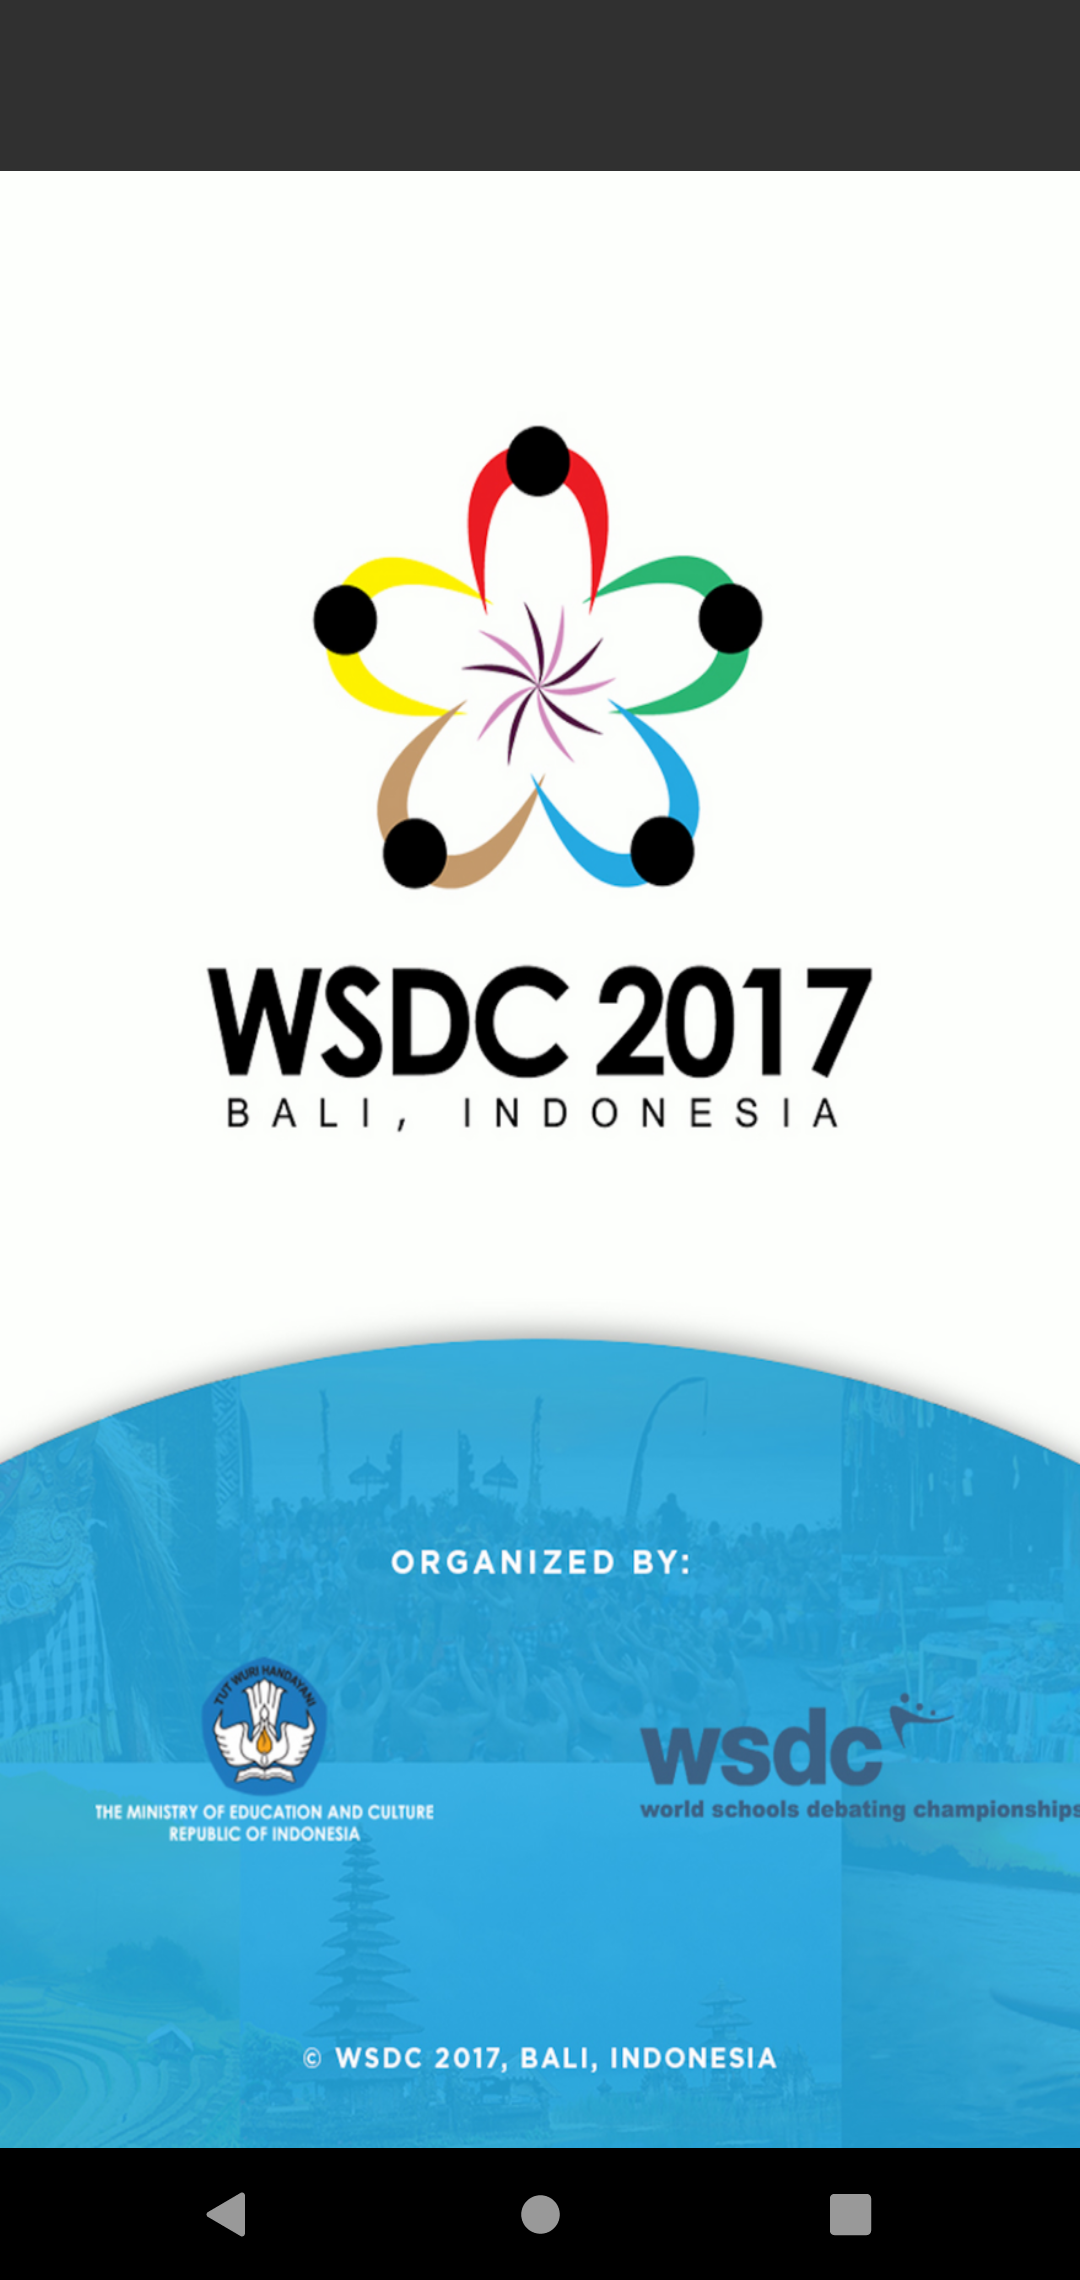
\includegraphics[width=\textwidth]{Gambar/SSSplashScreen.png}
         \caption{\textit{Splash Screen Page} Terbaru}
         \label{fig:ssSplashScreen}
     \end{subfigure}
     \hspace*{0.5in}
     \begin{subfigure}[b]{0.3\textwidth}
         \centering
         
\includegraphics[width=\textwidth]{Gambar/SplashScreenOld.png}
         \caption{\textit{Splash Screen Page} Terdahulu}
         \label{fig:ssSplashScreenOld}
     \end{subfigure}
        \caption{Tangkapan Layar Halaman Splash Screen Aplikasi WSDC 2017 Bali}
        \label{fig:ssApk1}
\end{figure}

\begin{figure}[H]
     \centering
     \begin{subfigure}[b]{0.3\textwidth}
         \centering
         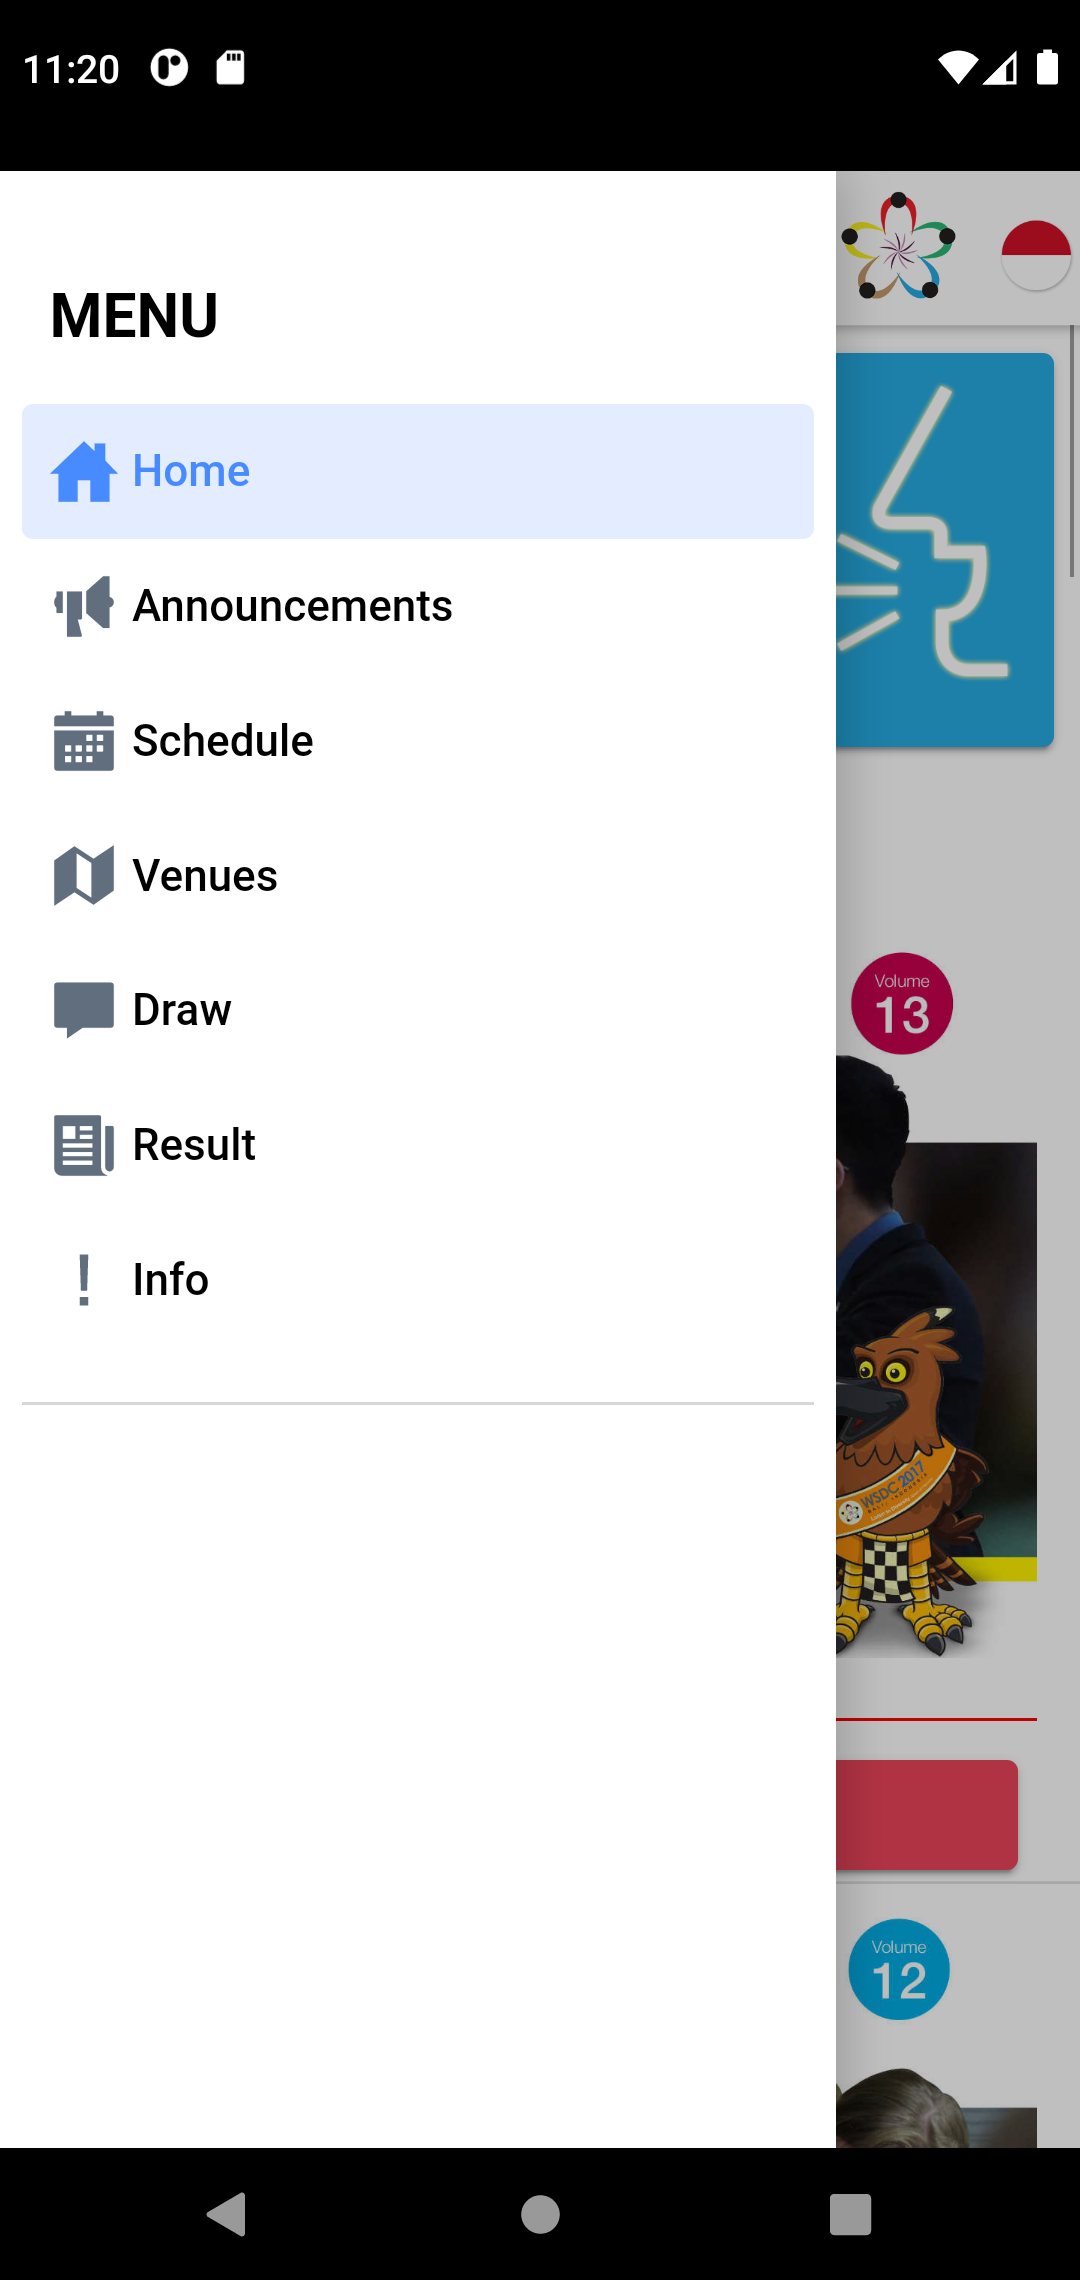
\includegraphics[width=\textwidth]{Gambar/SSSidebar.png}
         \caption{\textit{Sidemenu} Terbaru}
         \label{fig:ssSidebar}
     \end{subfigure}
     \hspace*{0.5in}
     \begin{subfigure}[b]{0.3\textwidth}
         \centering
         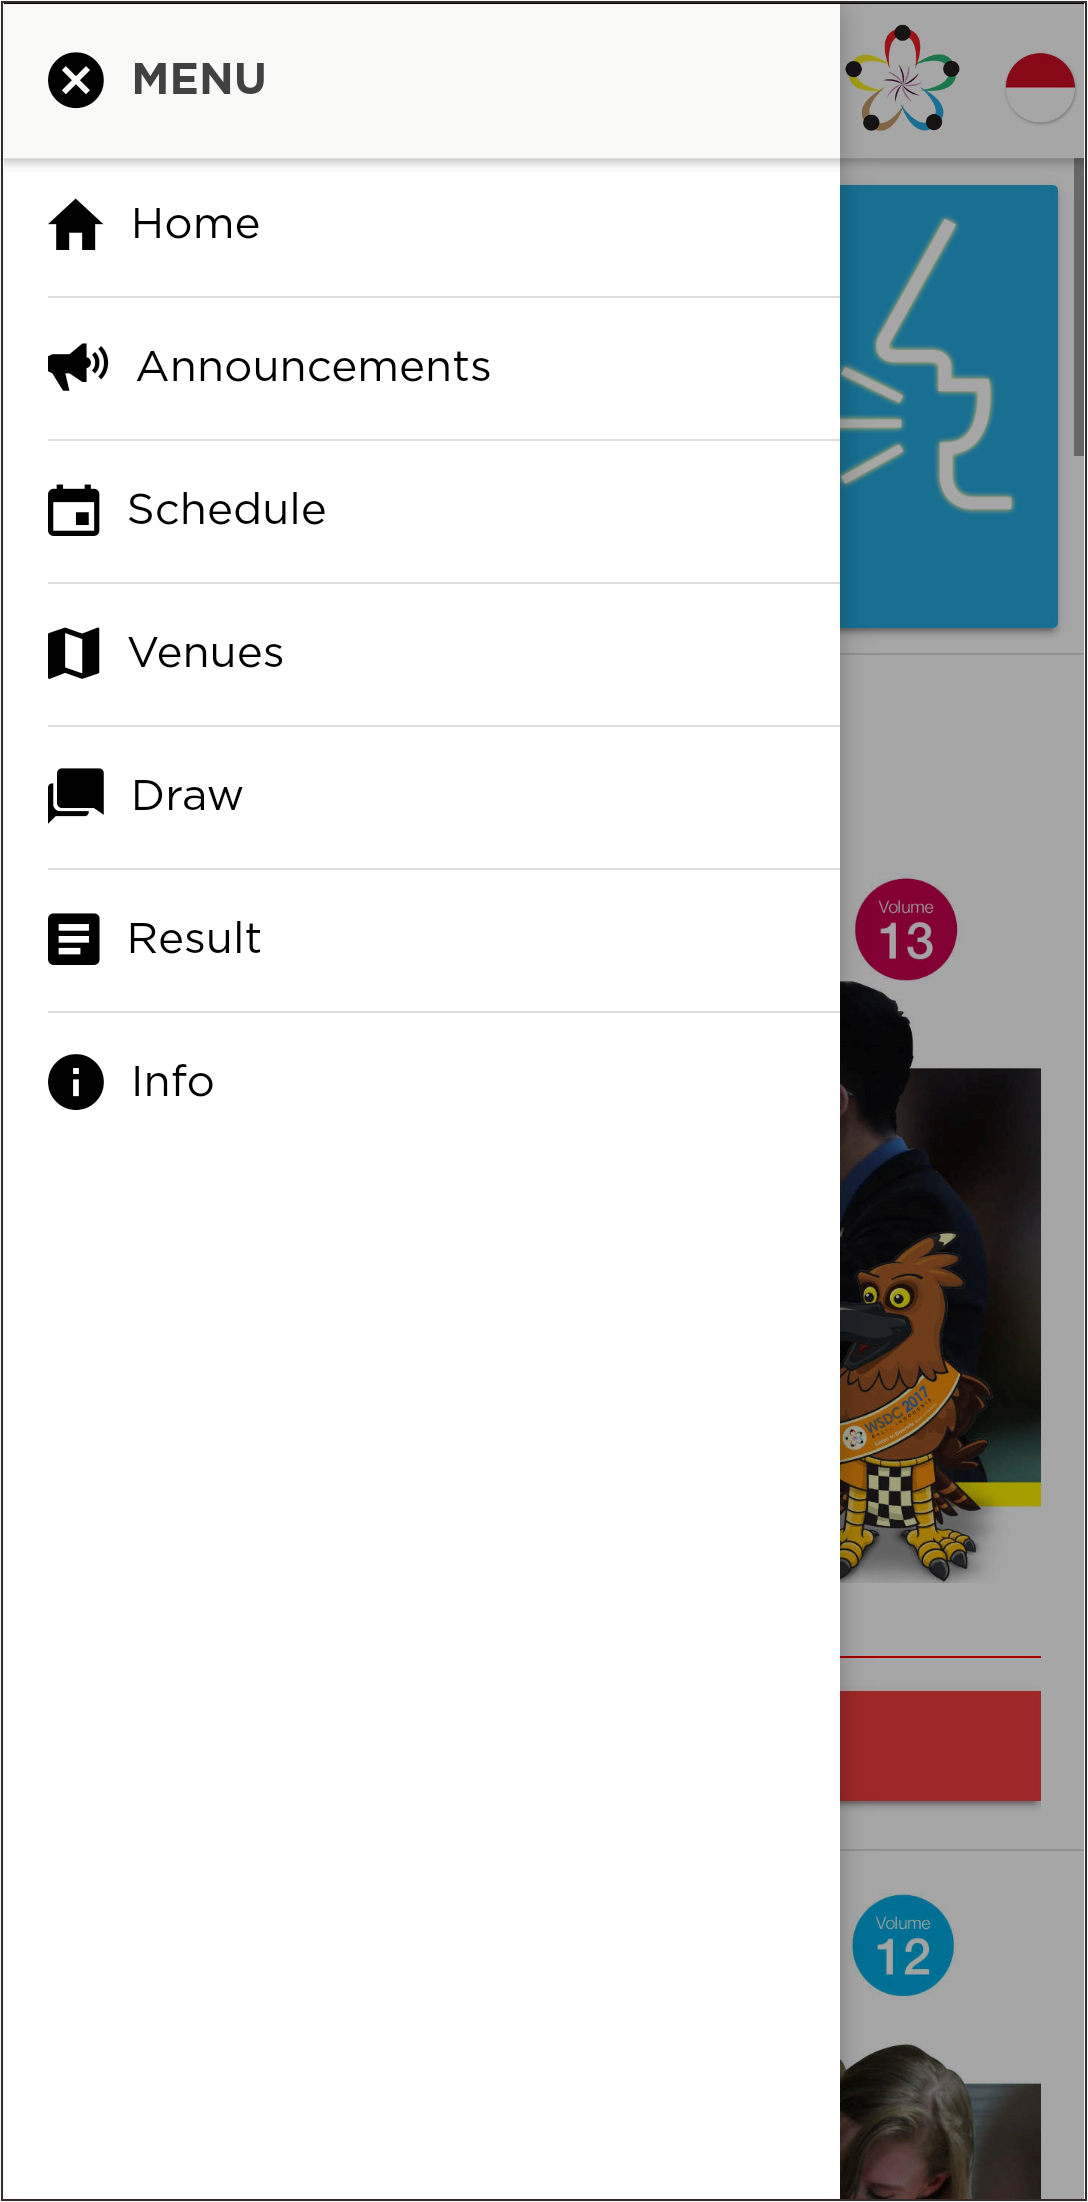
\includegraphics[width=\textwidth]{Gambar/SideBarOld.png}
         \caption{\textit{Sidemenu} Terdahulu}
         \label{fig:ssSidebarOld}
     \end{subfigure}
        \caption{Tangkapan Layar Sidemenu Aplikasi WSDC 2017 Bali}
        \label{fig:ssApk1}
\end{figure}


\begin{figure}[H]
     \centering
     \begin{subfigure}[b]{0.3\textwidth}
         \centering
         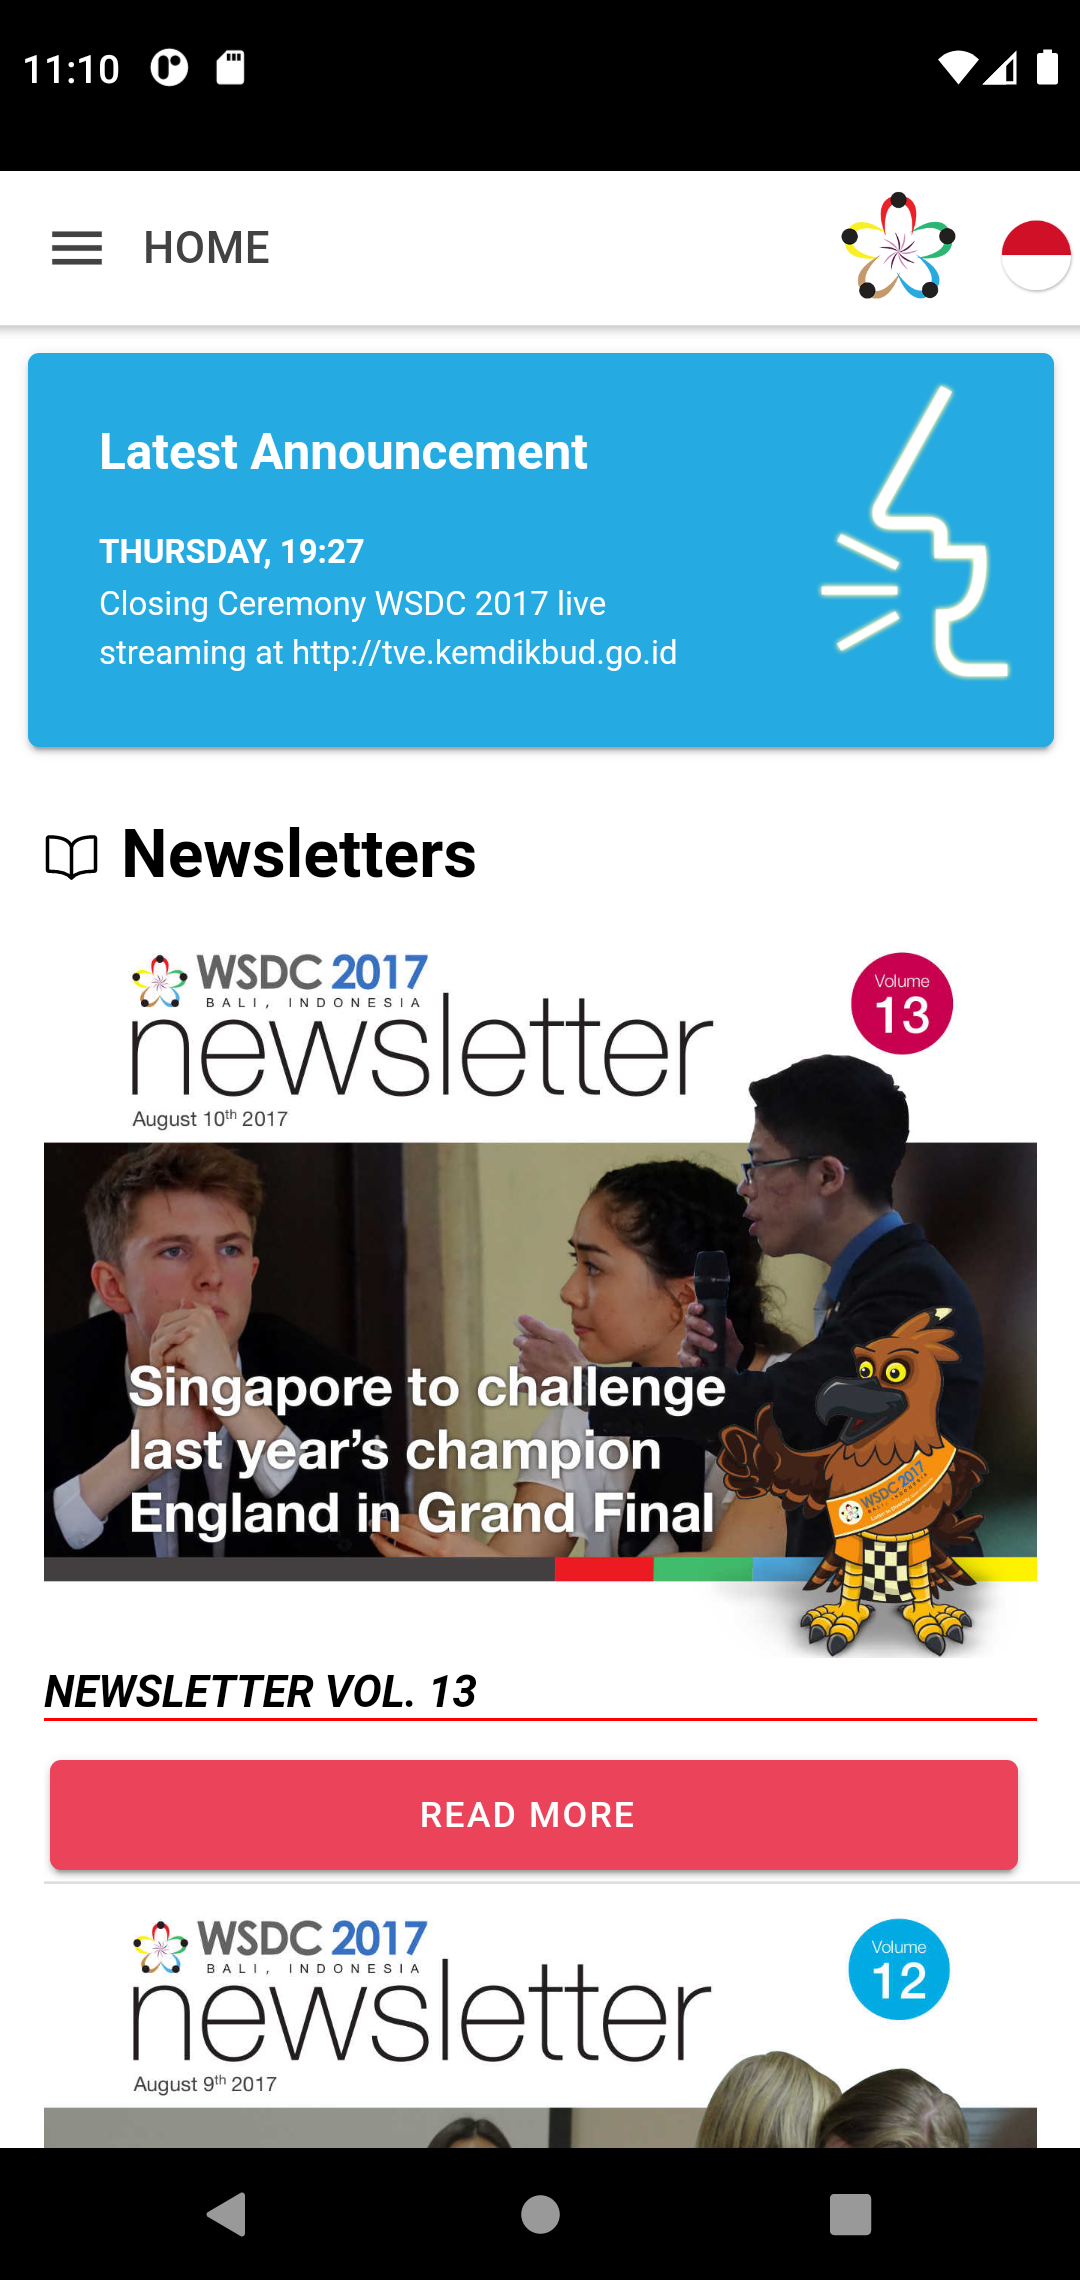
\includegraphics[width=\textwidth]{Gambar/SSHome.png}
         \caption{\textit{Home Page} Terbaru}
         \label{fig:ssHome}
     \end{subfigure}
     \hspace*{0.5in}
     \begin{subfigure}[b]{0.3\textwidth}
         \centering
         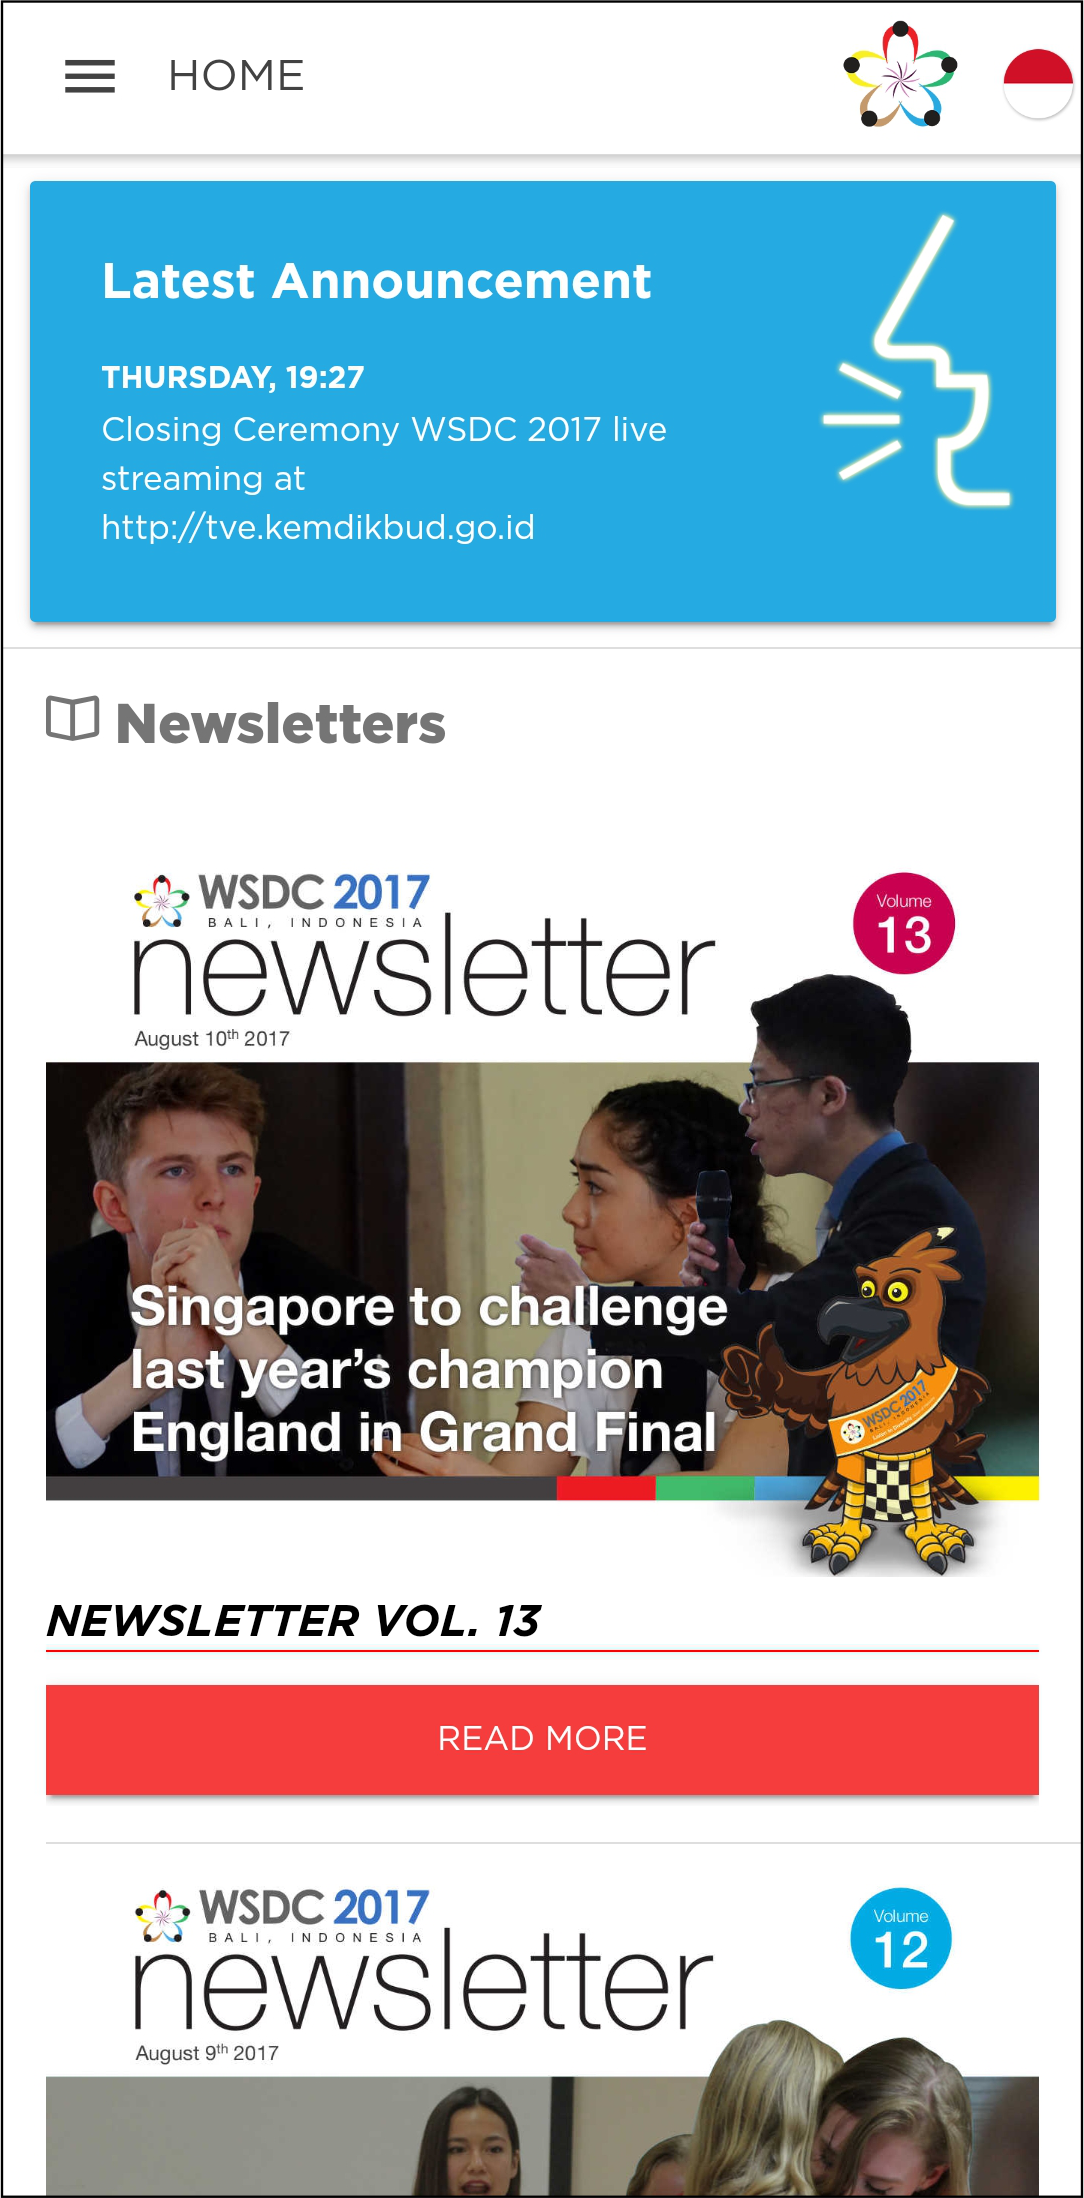
\includegraphics[width=\textwidth]{Gambar/HomePage.png}
         \caption{\textit{Home Page} Terdahulu}
         \label{fig:ssHomeOld}
     \end{subfigure}
        \caption{Tangkapan Layar Halaman Home Aplikasi WSDC 2017 Bali}
        \label{fig:ssApk1}
\end{figure}


\begin{figure}[H]
     \centering
     \begin{subfigure}[b]{0.3\textwidth}
         \centering
         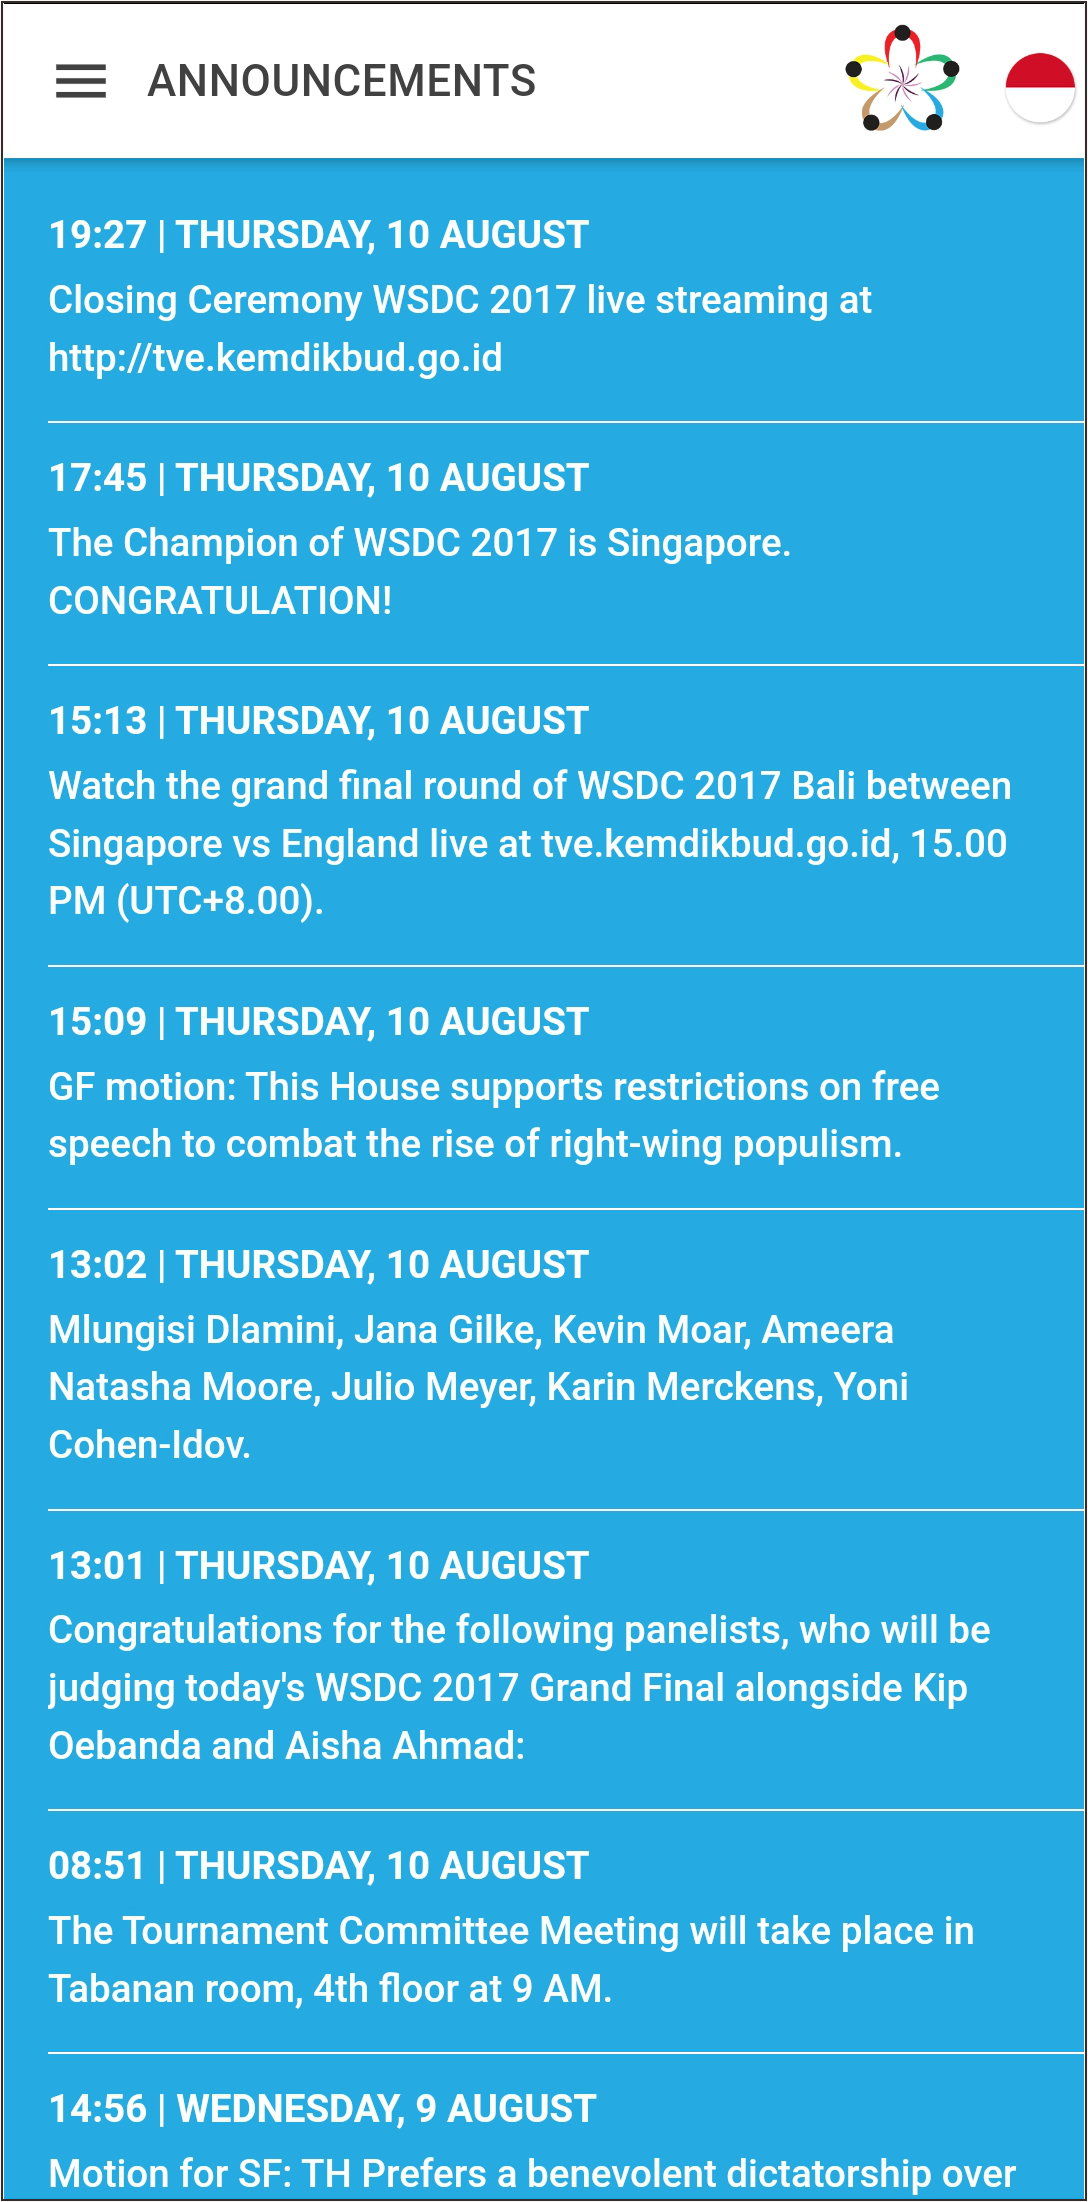
\includegraphics[width=\textwidth]{Gambar/SSAnnuncements.png}
         \caption{\textit{Announcements Page} Terbaru}
         \label{fig:ssAnnouncements}
     \end{subfigure}
     \hspace*{0.5in}
     \begin{subfigure}[b]{0.3\textwidth}
         \centering
         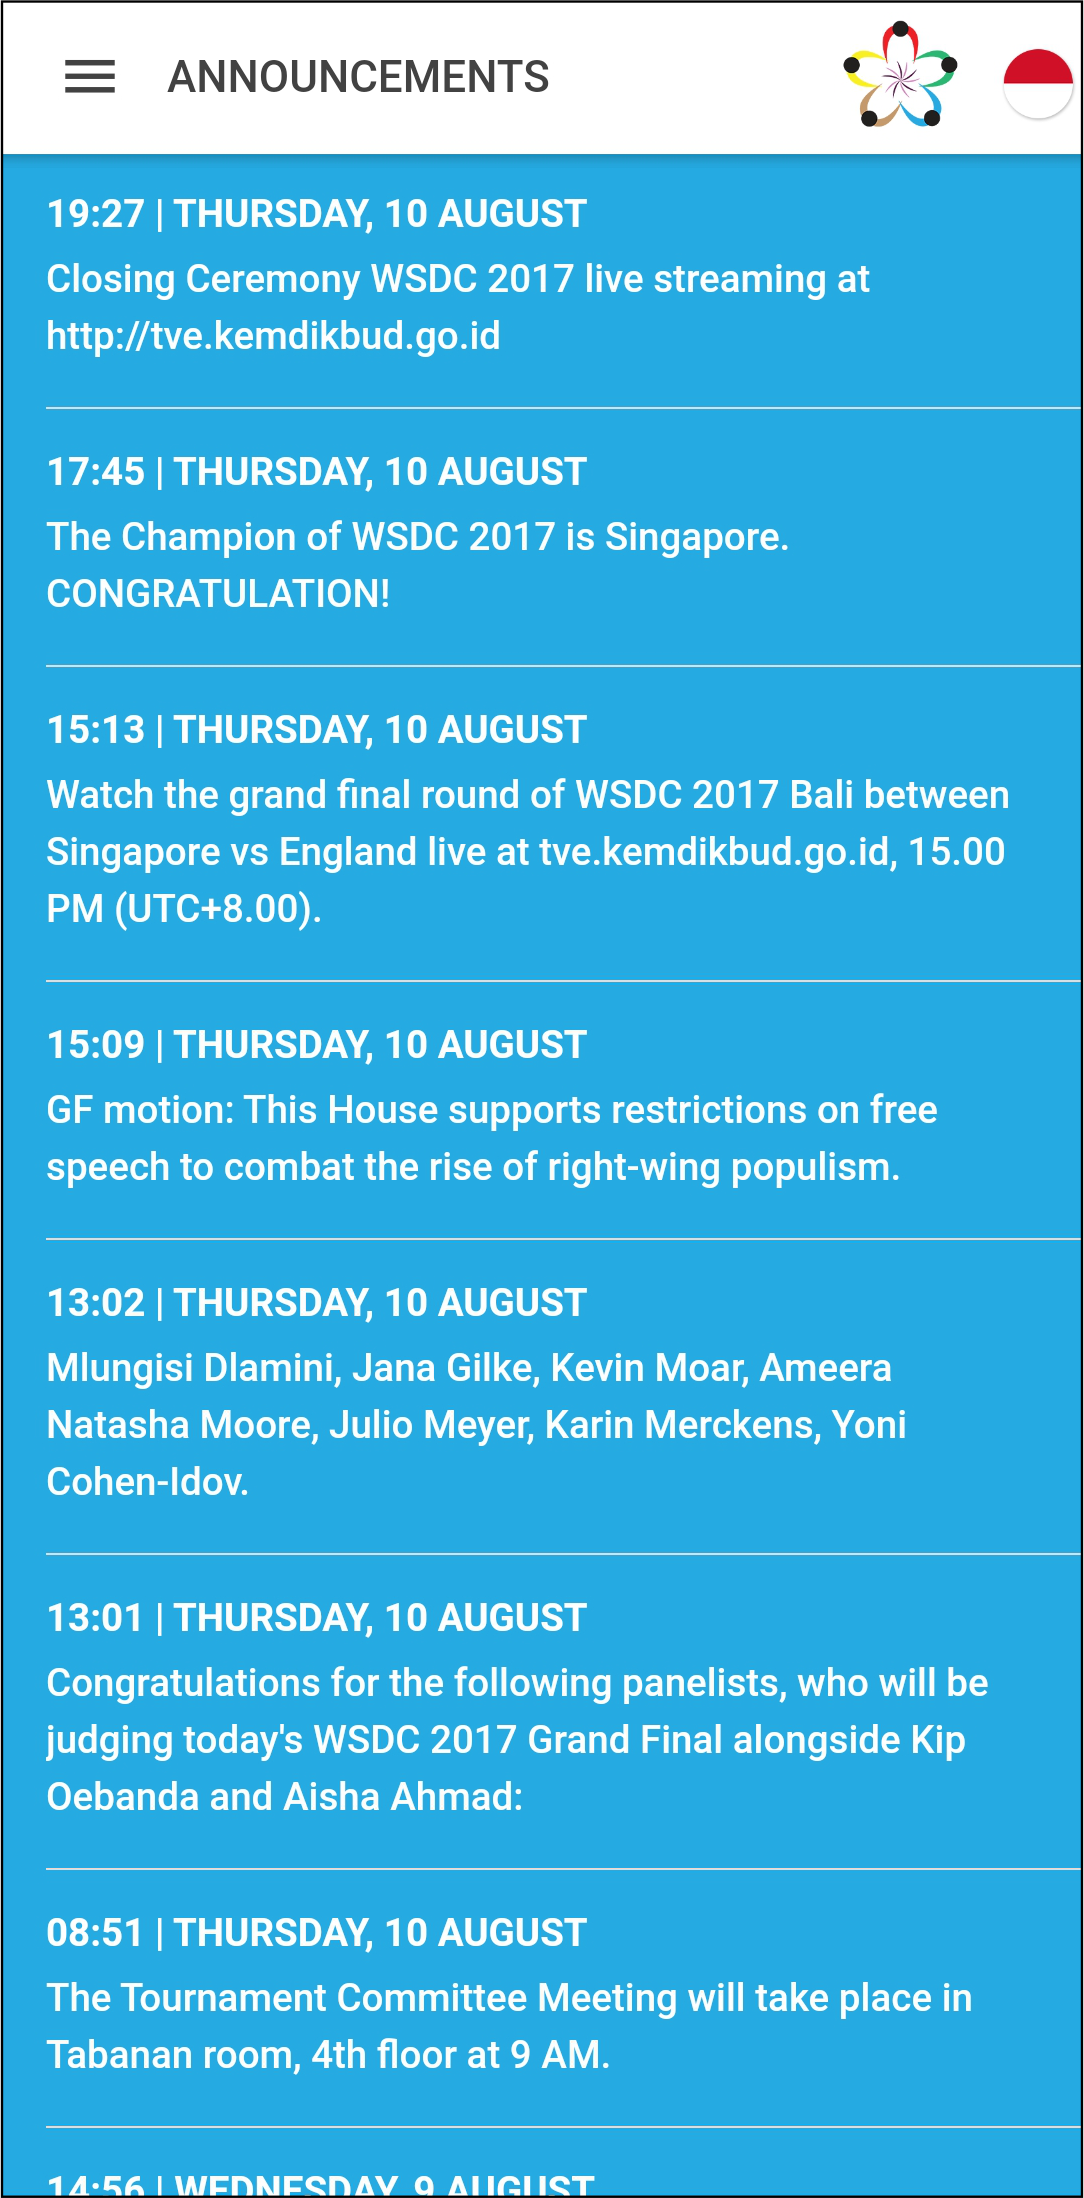
\includegraphics[width=\textwidth]{Gambar/AnnouncementsPage.png}
         \caption{\textit{Announcements Page} Terdahulu}
         \label{fig:ssAnnouncementsOld}
     \end{subfigure}
        \caption{Tangkapan Layar Halaman \textit{Announcements} Aplikasi WSDC 2017 Bali}
        \label{fig:ssApk1}
\end{figure}


\begin{figure}[H]
     \centering
     \begin{subfigure}[b]{0.3\textwidth}
         \centering
         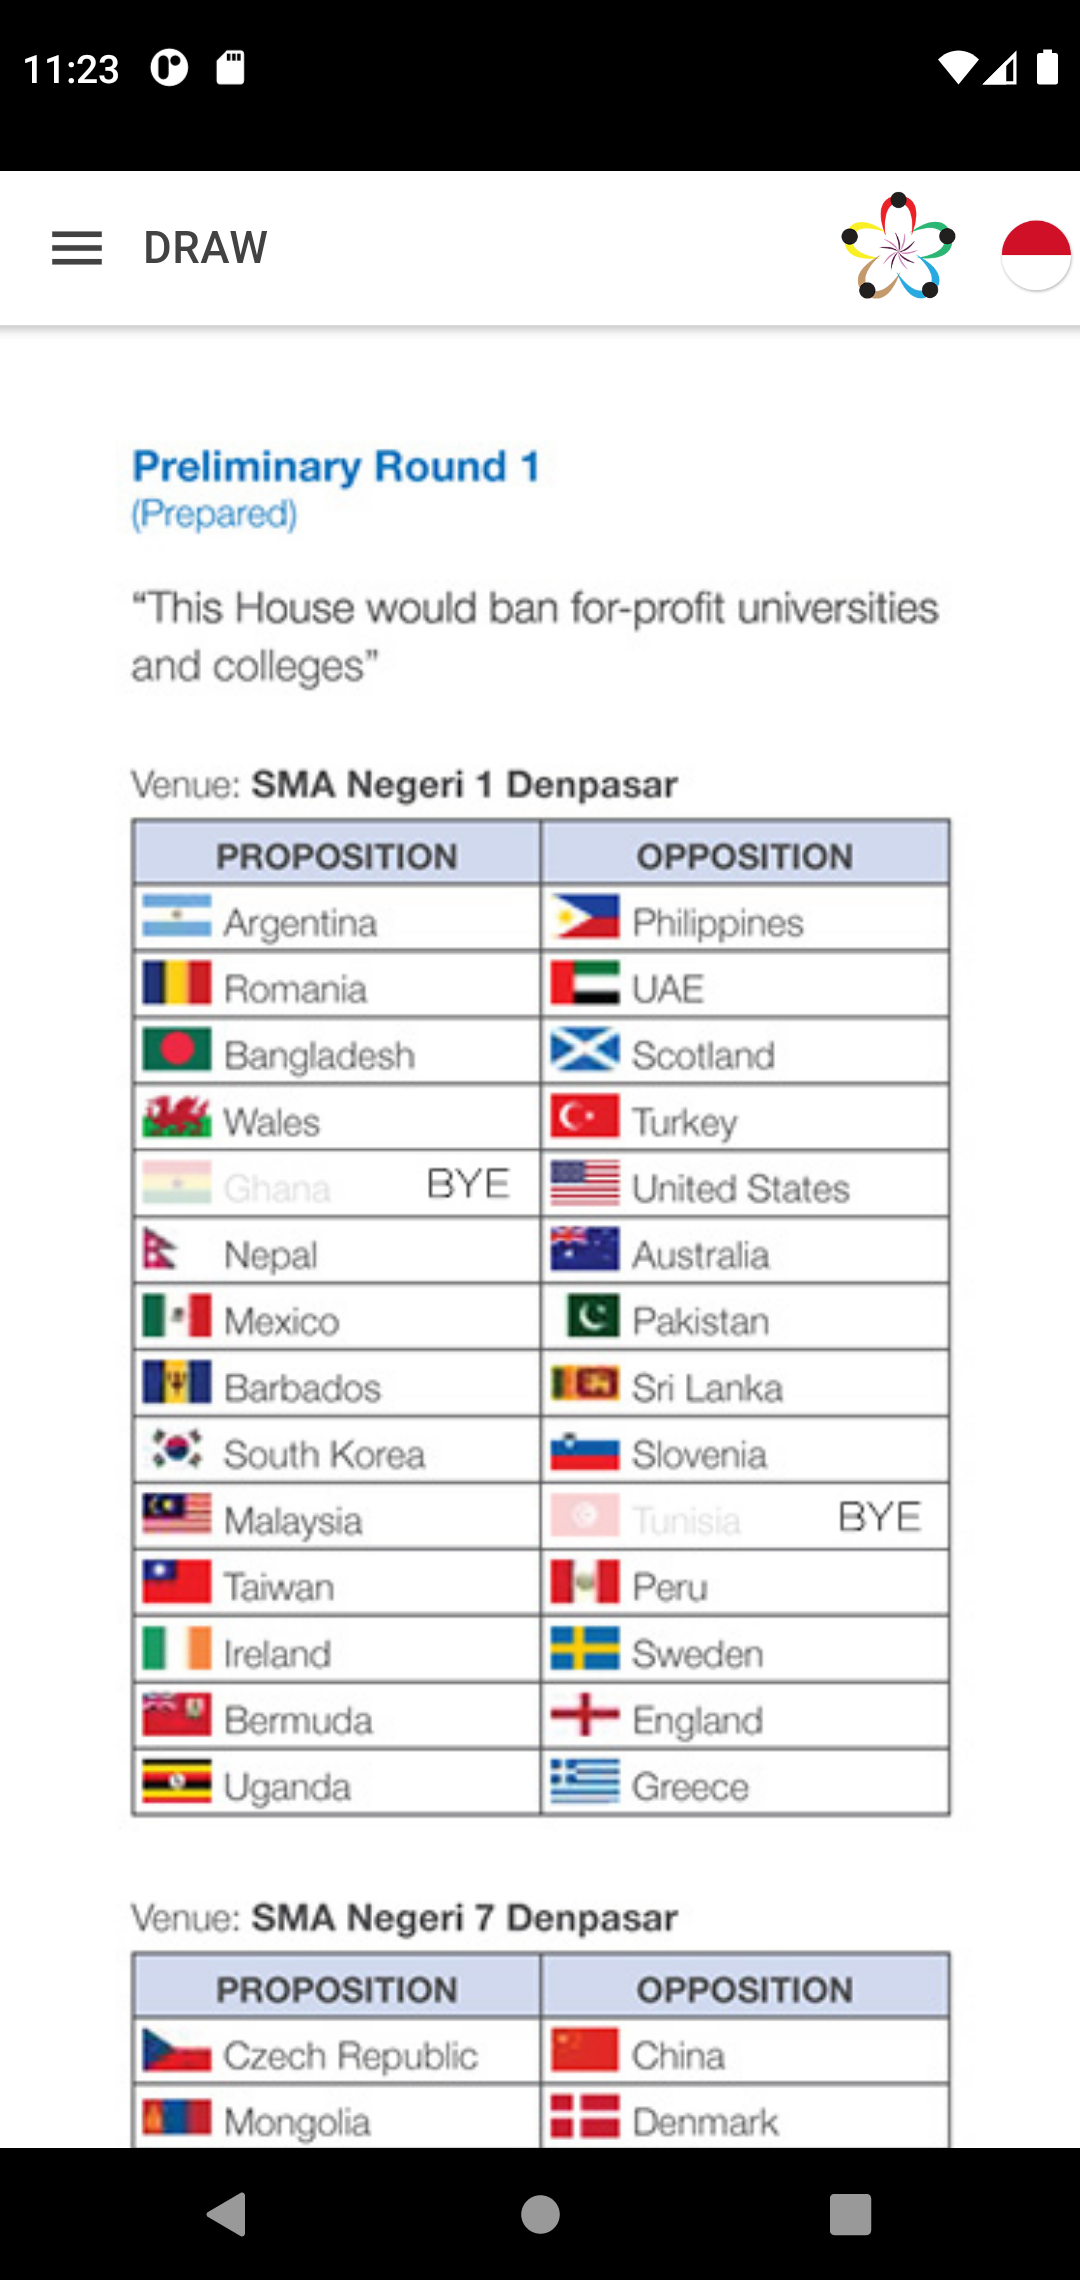
\includegraphics[width=\textwidth]{Gambar/SSDraw.png}
         \caption{\textit{Draw Page} Terbaru}
         \label{fig:ssDraw}
     \end{subfigure}
     \hspace*{0.5in}
     \begin{subfigure}[b]{0.3\textwidth}
         \centering
         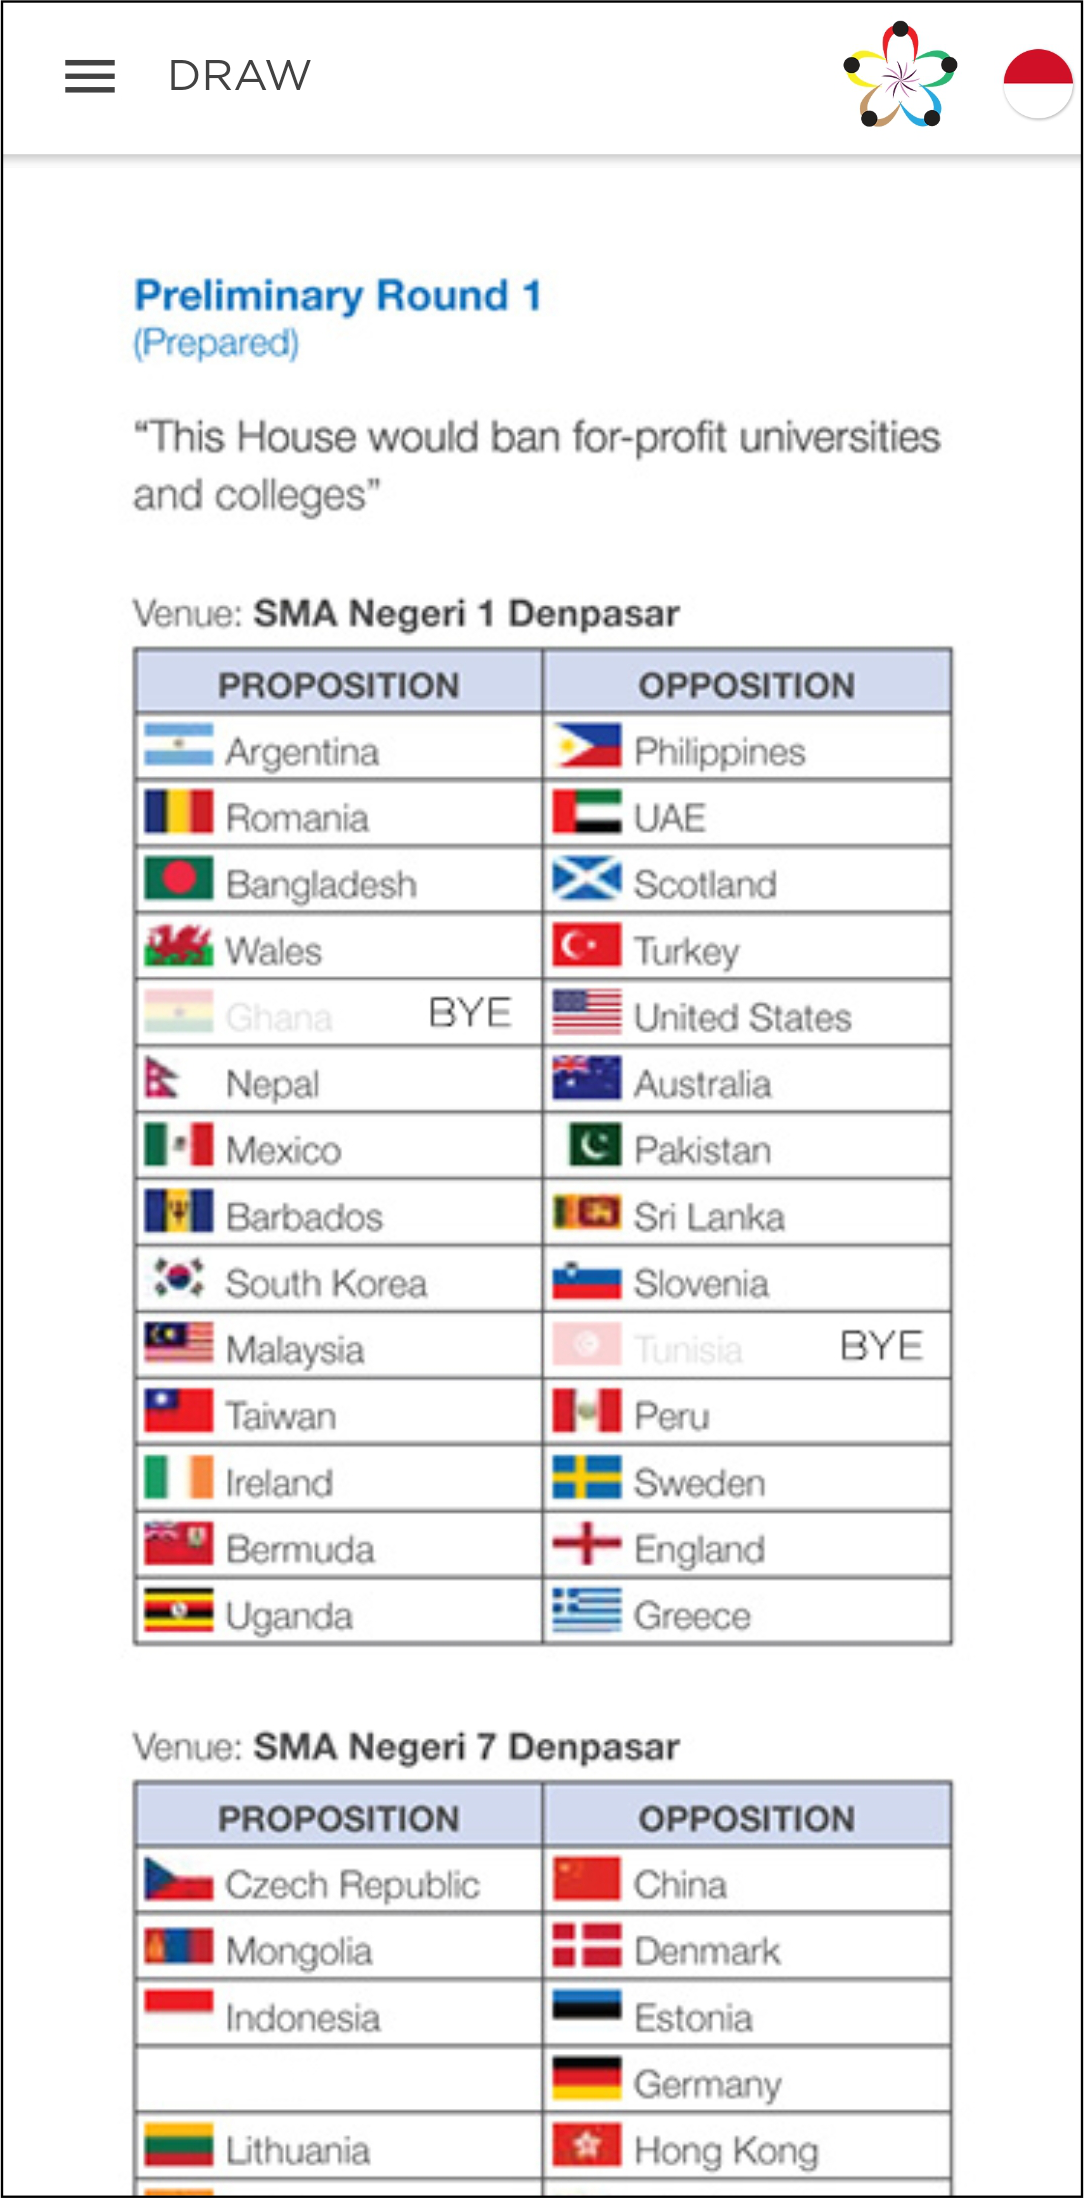
\includegraphics[width=\textwidth]{Gambar/DrawPage.png}
         \caption{\textit{Draw Page} Terdahulu}
         \label{fig:ssDrawOld}
     \end{subfigure}
        \caption{Tangkapan Layar Halaman \textit{Draw} Aplikasi WSDC 2017 Bali}
        \label{fig:ssApk1}
\end{figure}


\begin{figure}[H]
     \centering
     \begin{subfigure}[b]{0.3\textwidth}
         \centering
         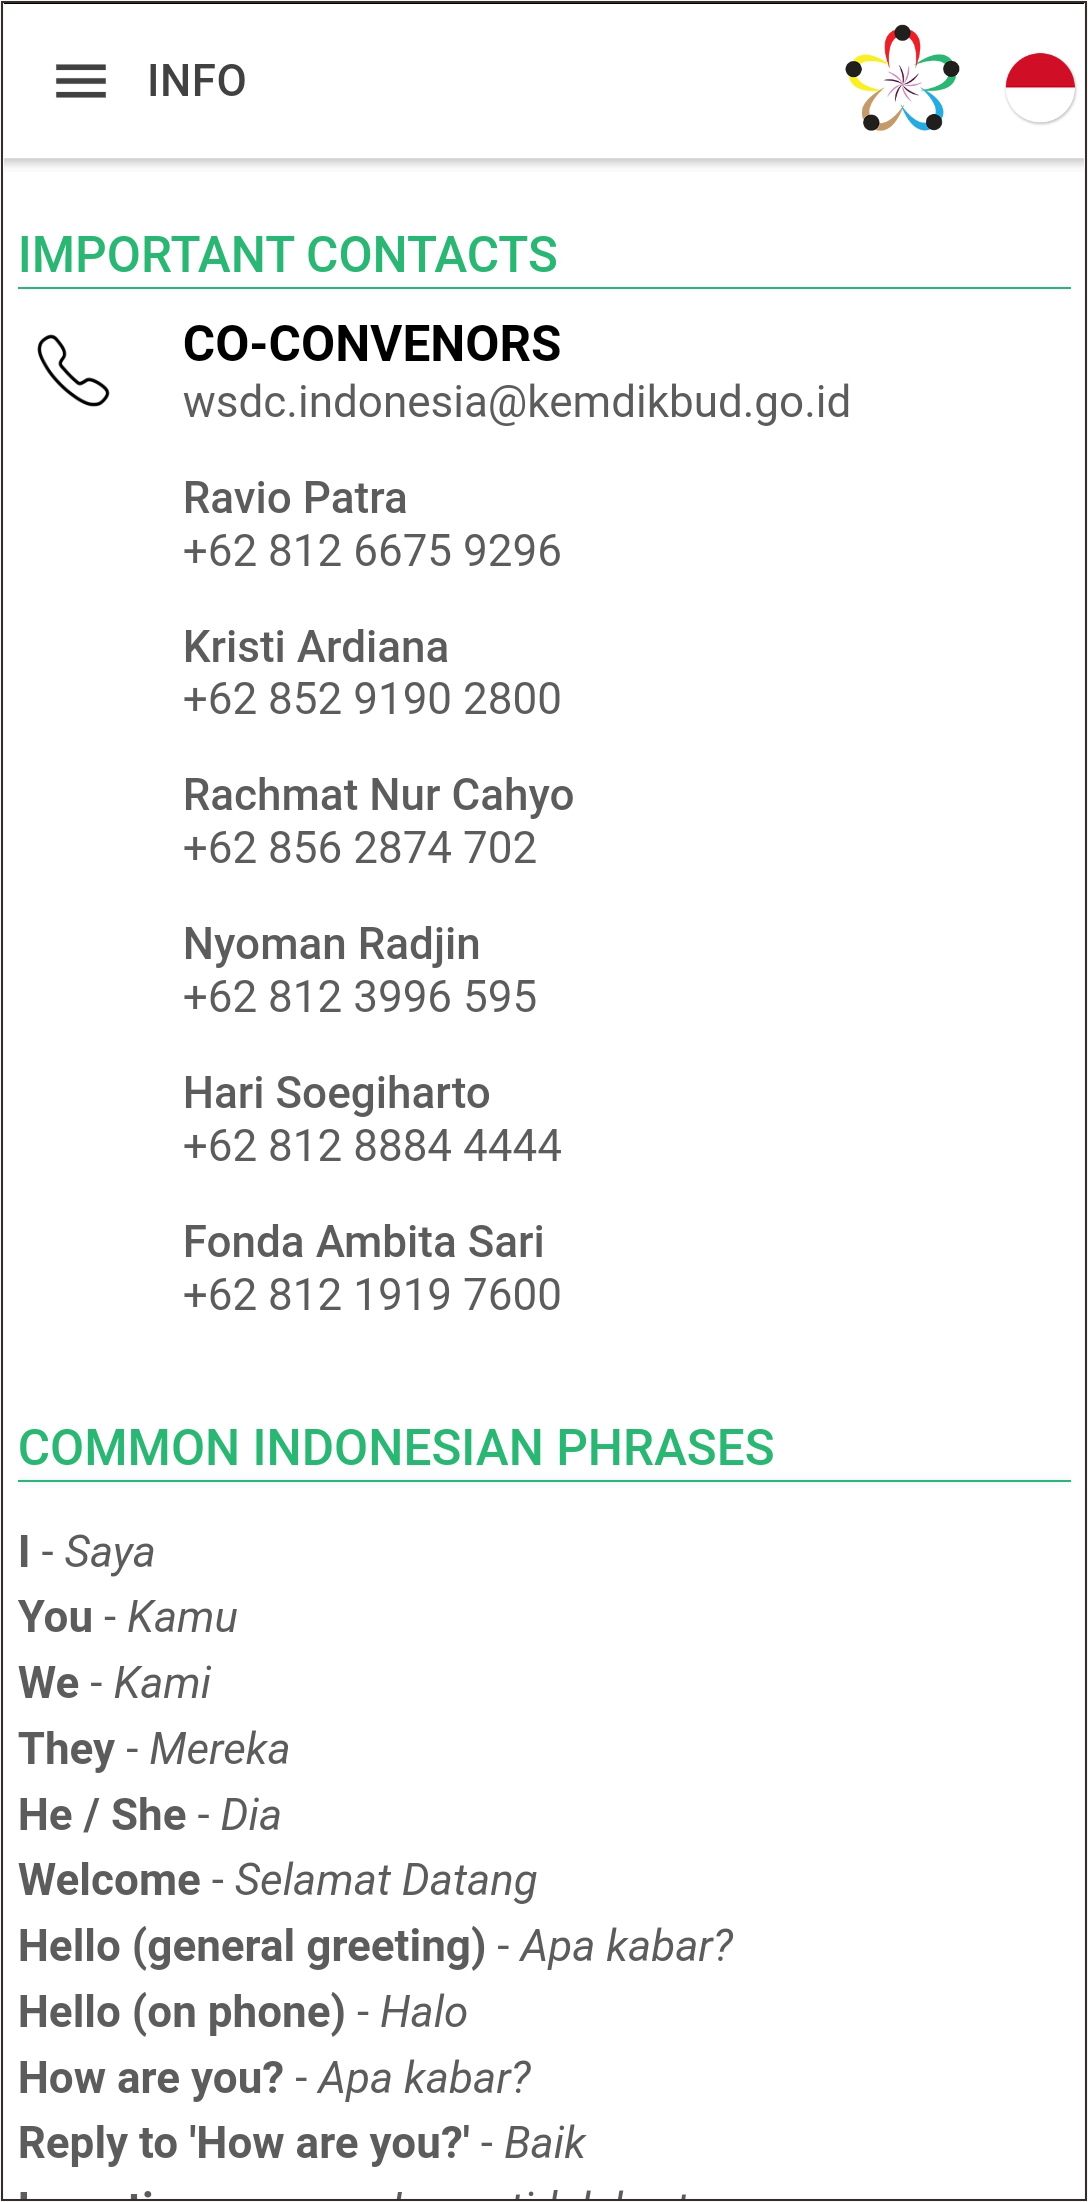
\includegraphics[width=\textwidth]{Gambar/SSInfo.png}
         \caption{Info \textit{Page} Terbaru}
         \label{fig:ssInfo}
     \end{subfigure}
     \hspace*{0.5in}
     \begin{subfigure}[b]{0.3\textwidth}
         \centering
         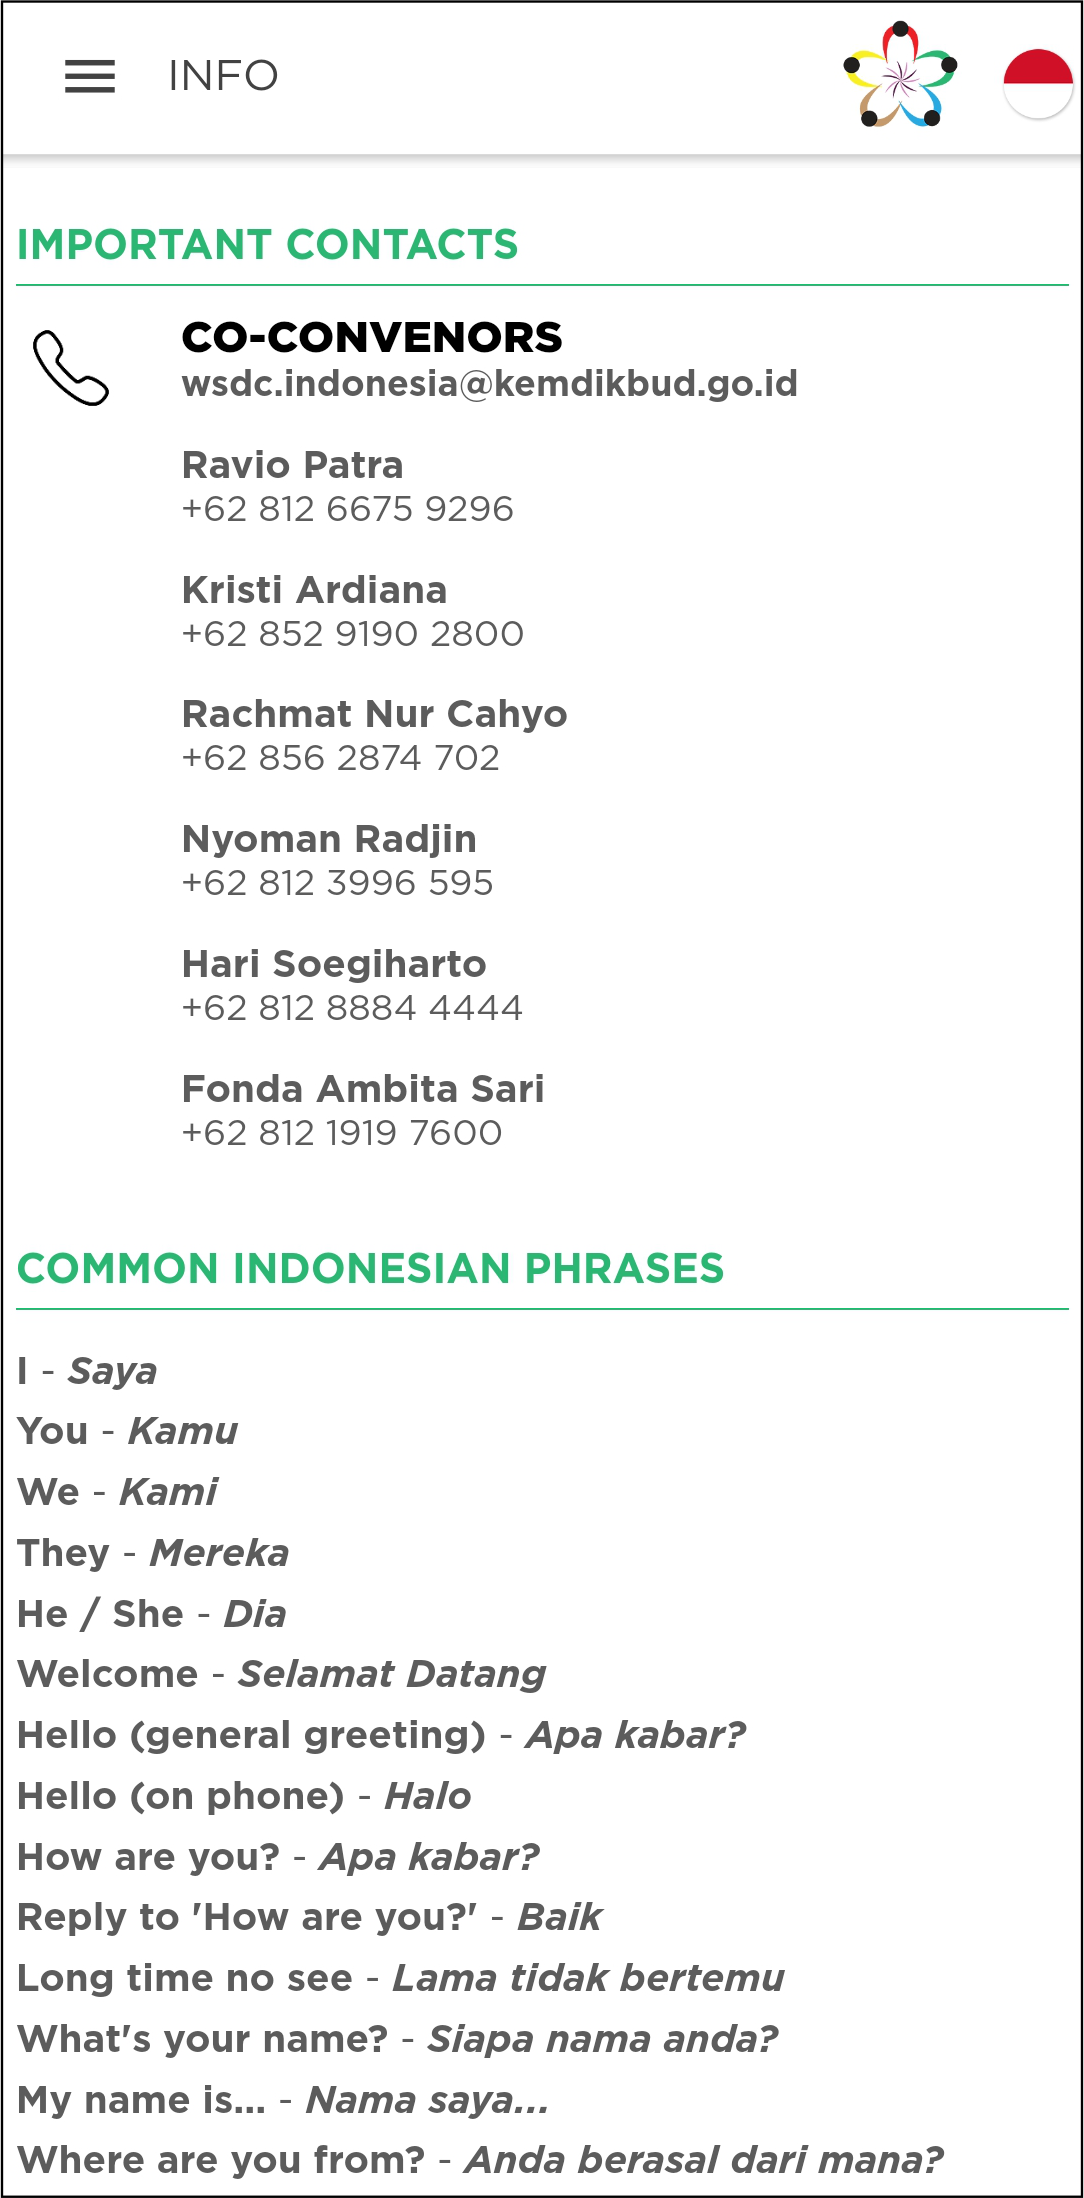
\includegraphics[width=\textwidth]{Gambar/InfoPage.png}
         \caption{Info \textit{Page} Terdahulu}
         \label{fig:ssInfoOld}
     \end{subfigure}
        \caption{Tangkapan Layar Halaman Info WSDC 2017 Bali}
        \label{fig:ssApk1}
\end{figure}


\begin{figure}[H]
     \centering
     \begin{subfigure}[b]{0.3\textwidth}
         \centering
         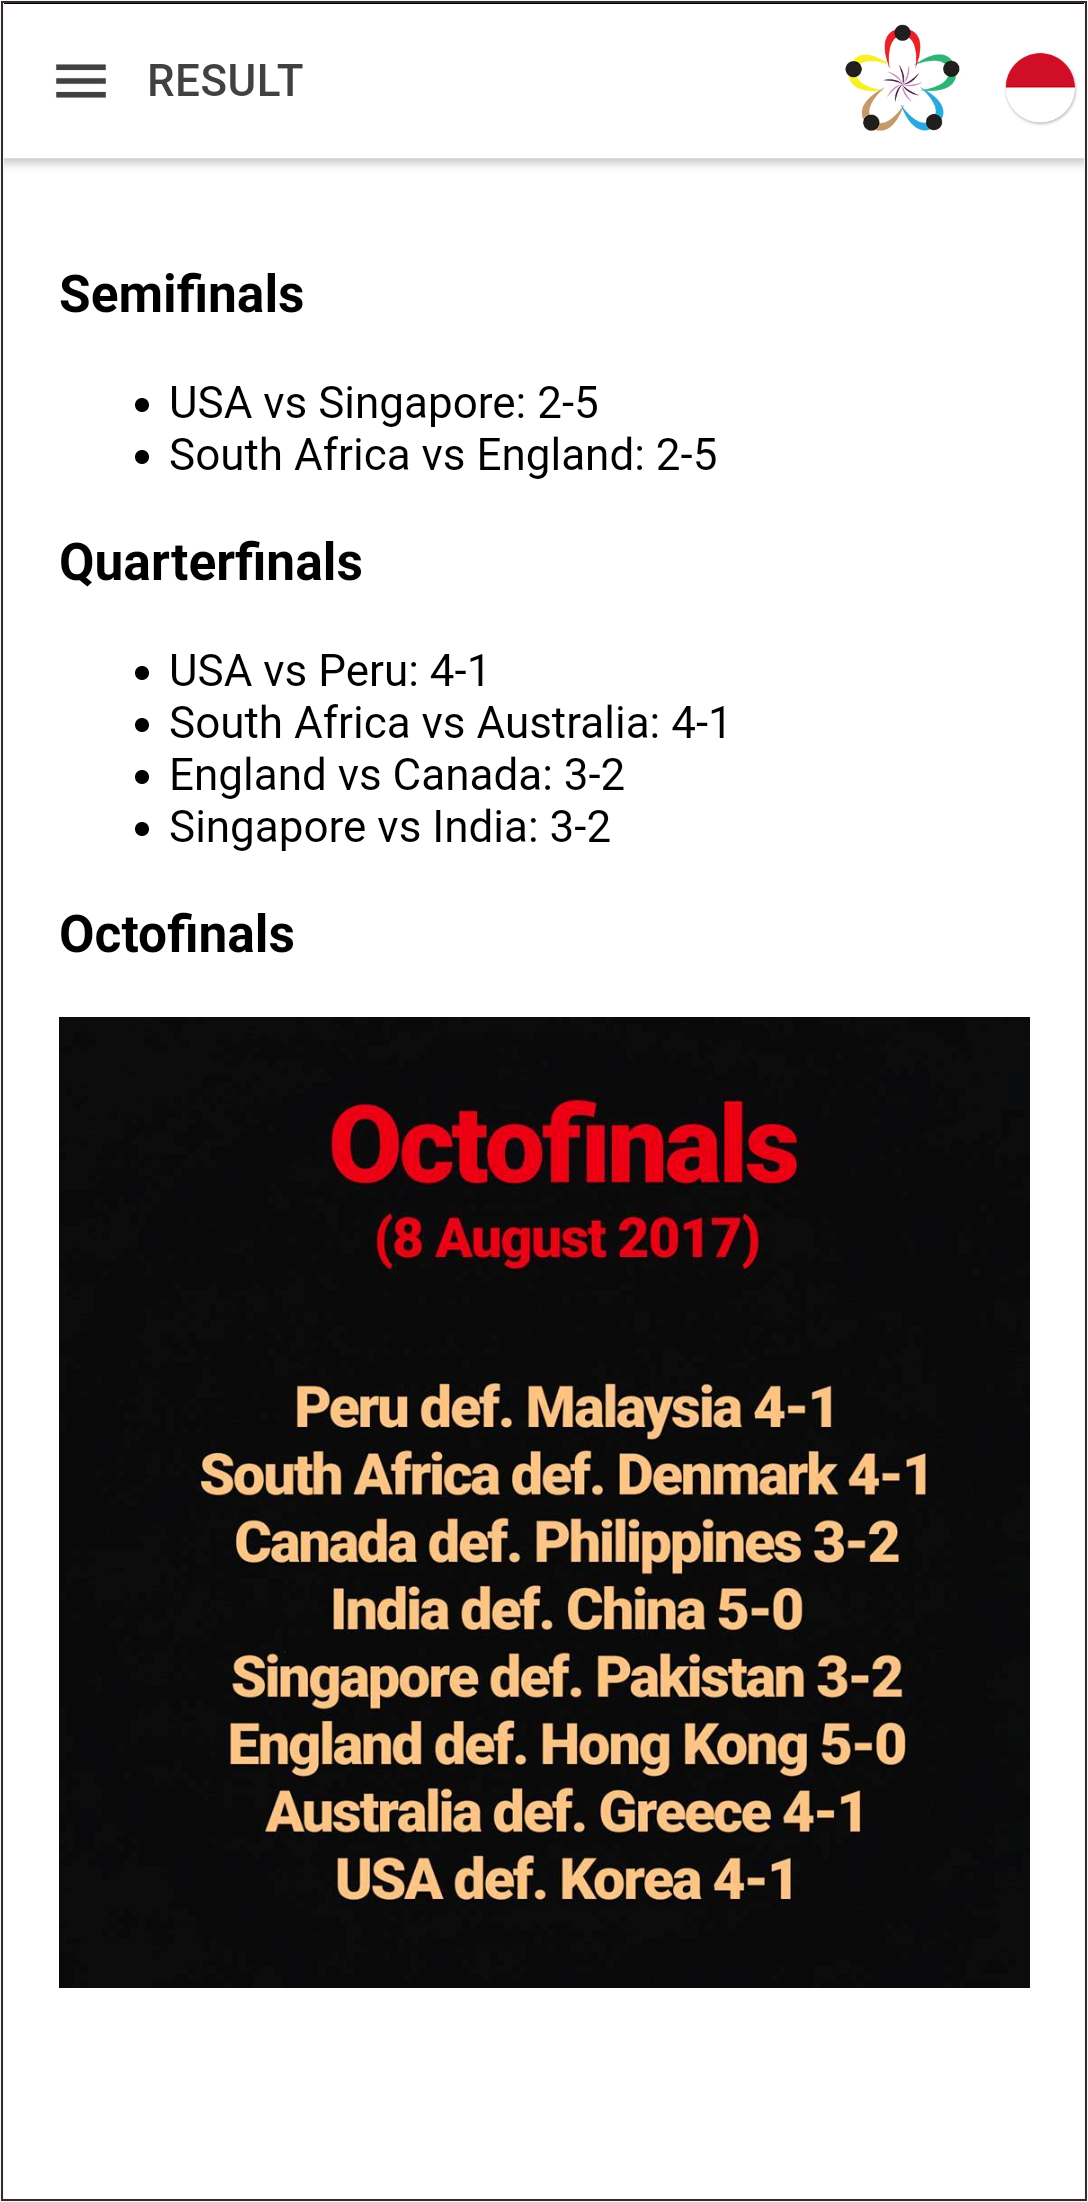
\includegraphics[width=\textwidth]{Gambar/SSResult.png}
         \caption{\textit{Result Page} Terbaru}
         \label{fig:ssResult}
     \end{subfigure}
     \hspace*{0.5in}
     \begin{subfigure}[b]{0.3\textwidth}
         \centering
         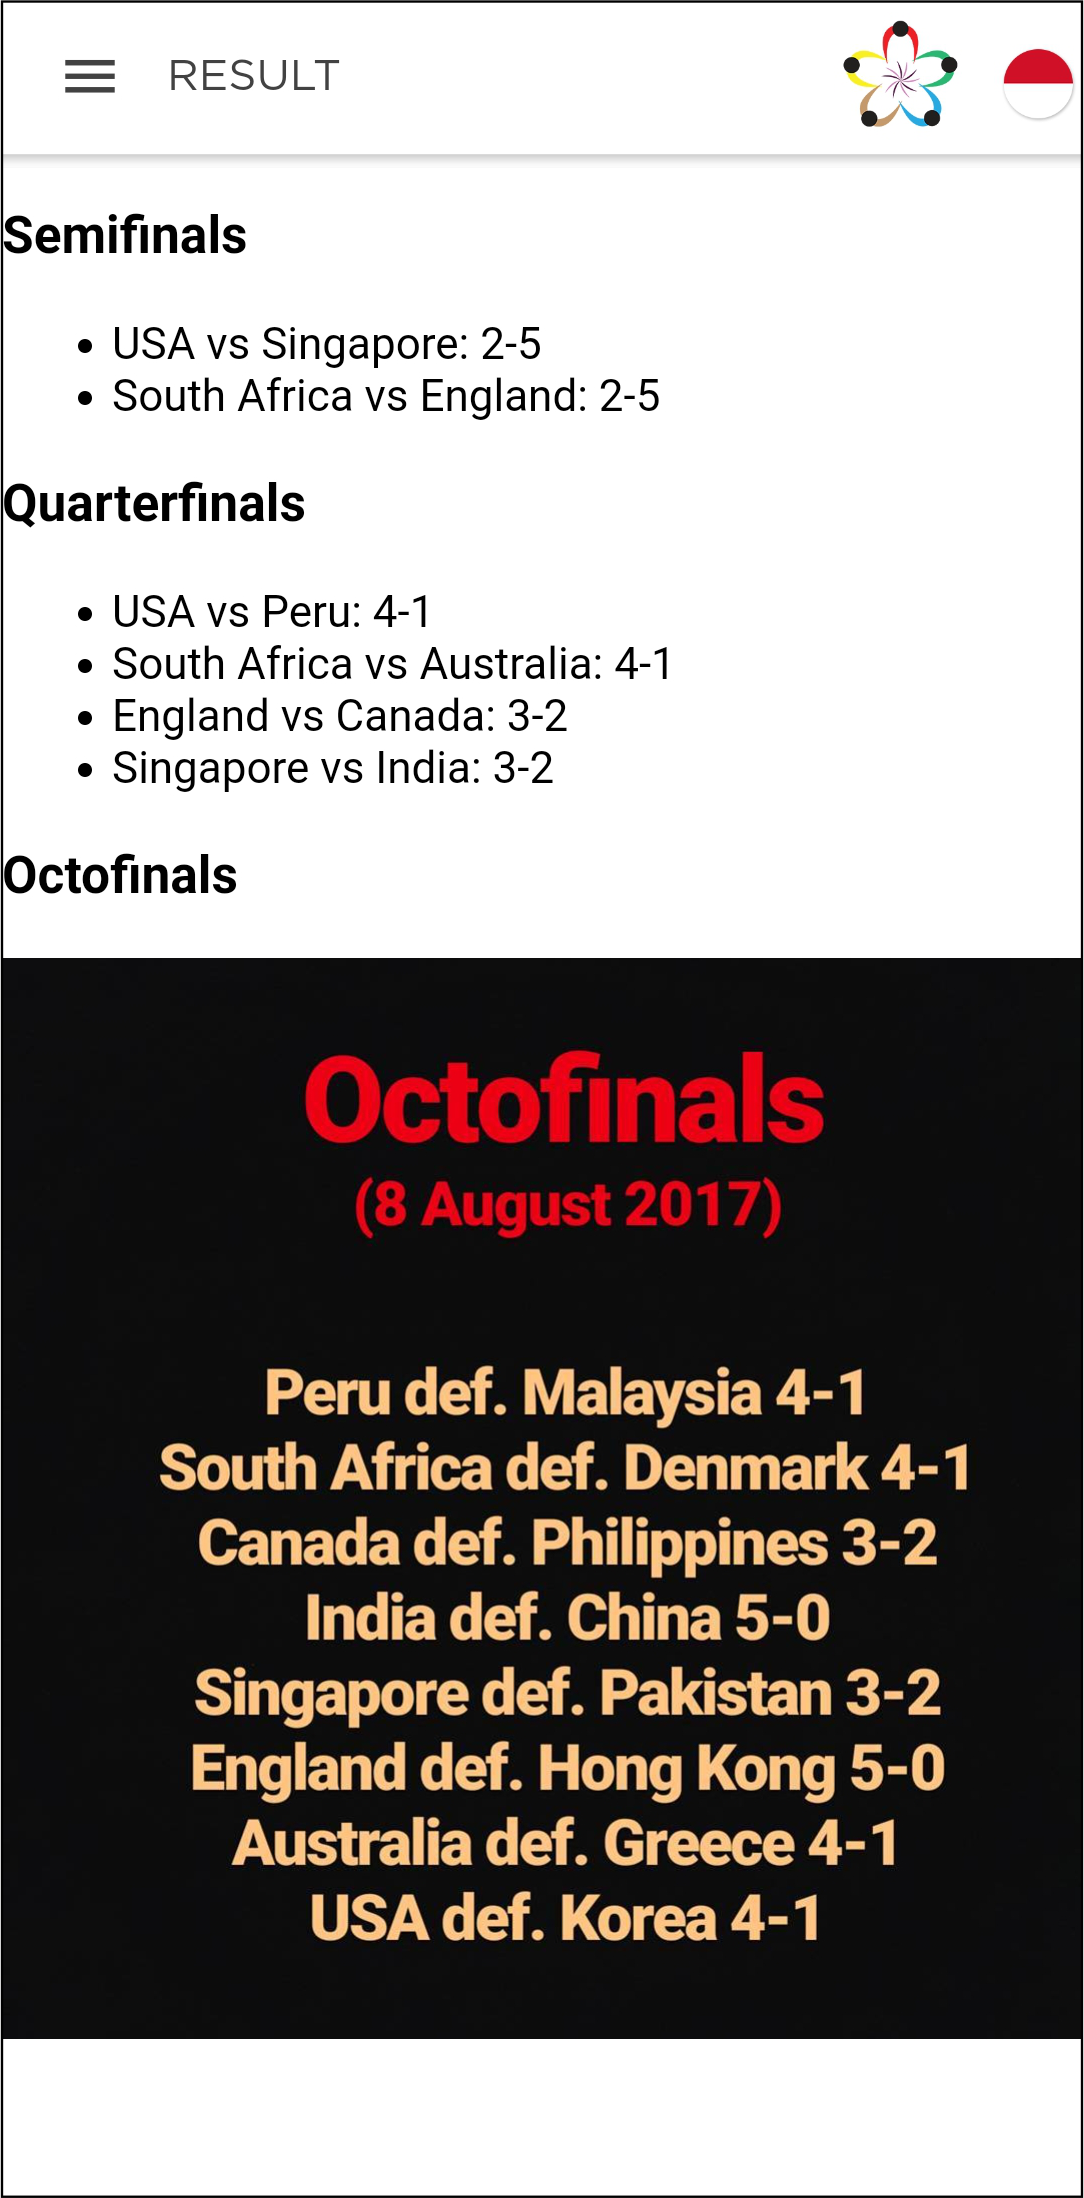
\includegraphics[width=\textwidth]{Gambar/ResultPage.png}
         \caption{\textit{Result Page} Terdahulu}
         \label{fig:ssResultOld}
     \end{subfigure}
        \caption{Tangkapan Layar Halaman \textit{Result} Aplikasi WSDC 2017 Bali}
        \label{fig:ssApk1}
\end{figure}


\begin{figure}[H]
     \centering
     \begin{subfigure}[b]{0.3\textwidth}
         \centering
         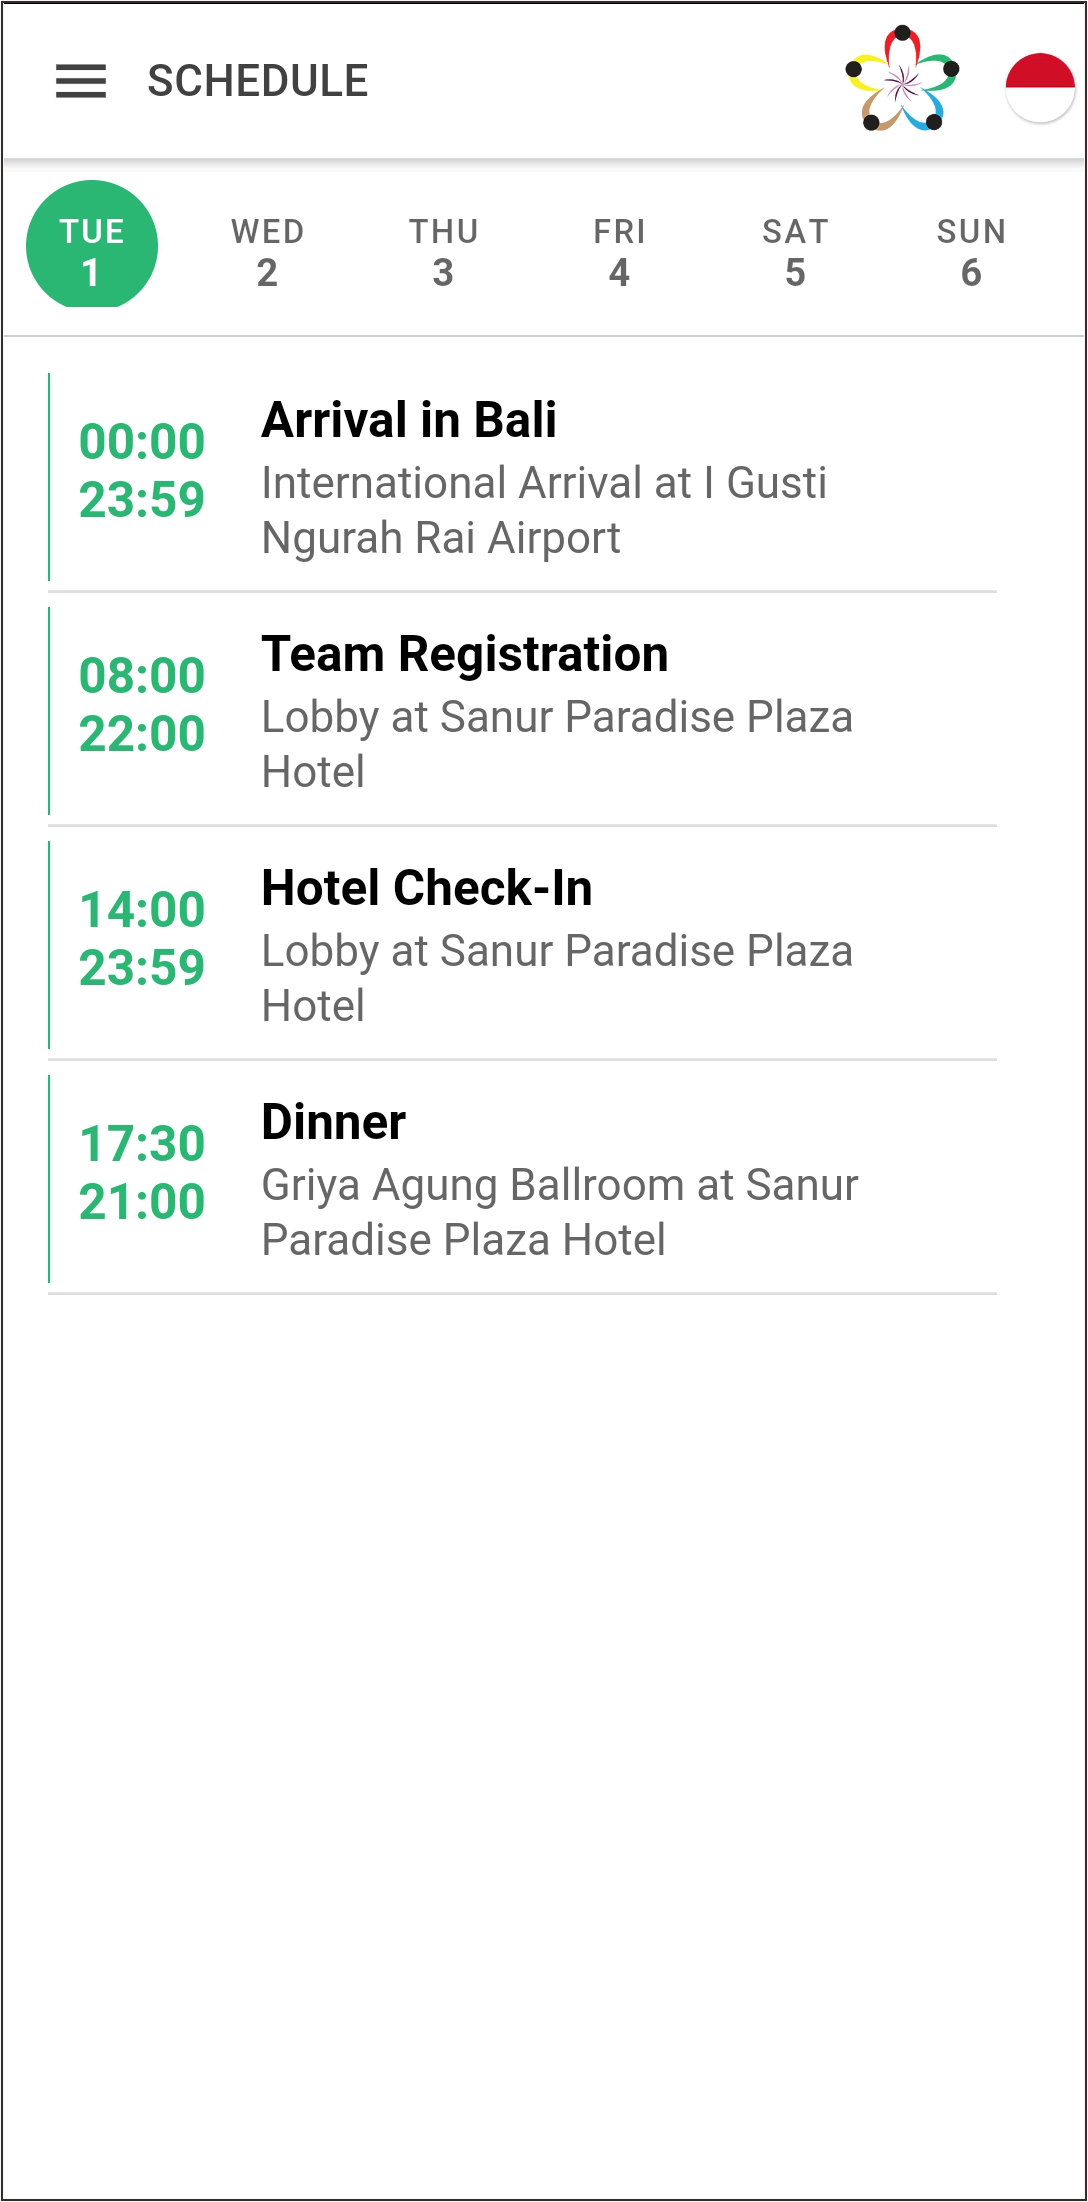
\includegraphics[width=\textwidth]{Gambar/SSSchedule.png}
         \caption{\textit{Schedule Page} Terbaru}
         \label{fig:ssSchedule}
     \end{subfigure}
     \hspace*{0.5in}
     \begin{subfigure}[b]{0.3\textwidth}
         \centering
         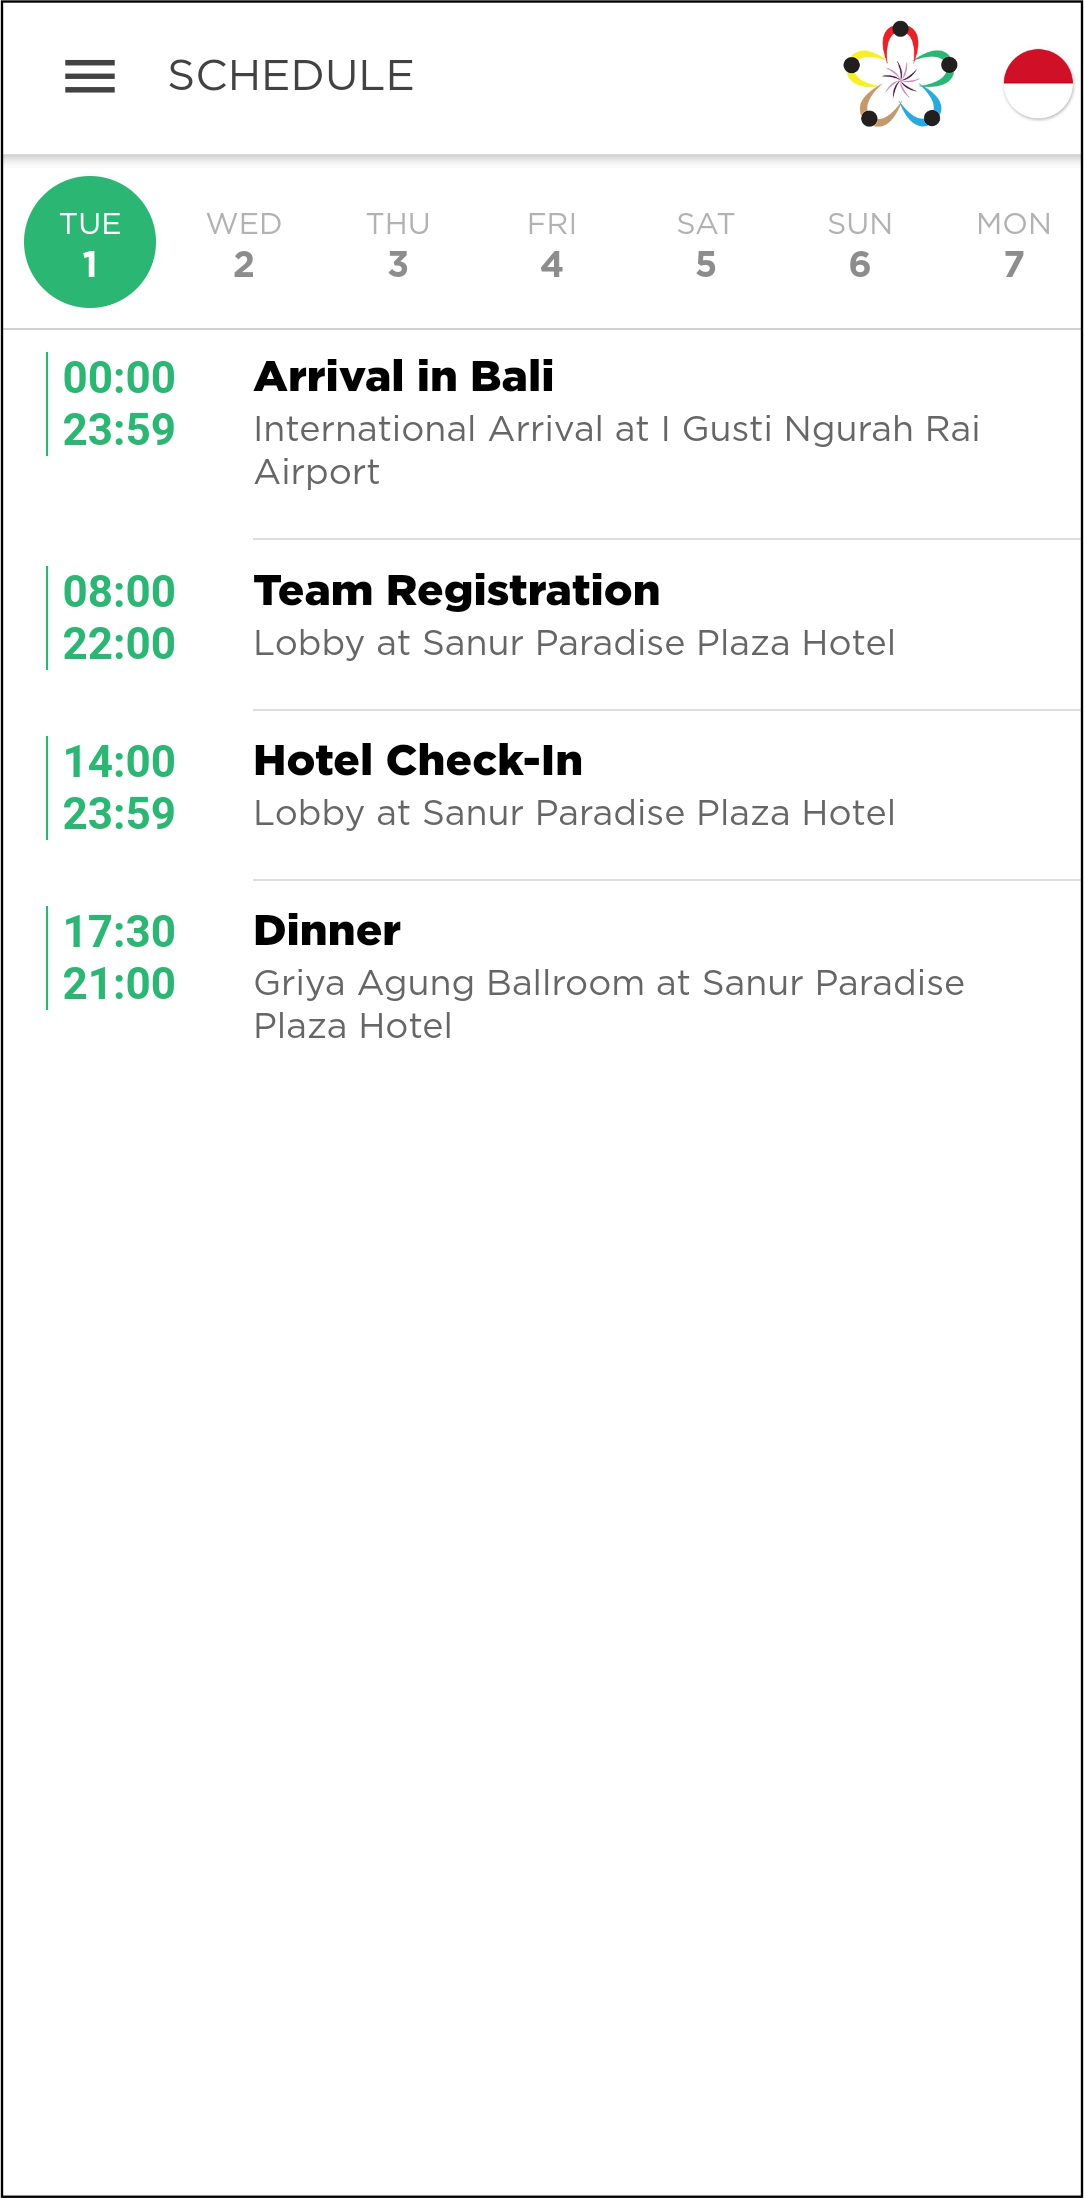
\includegraphics[width=\textwidth]{Gambar/SchedulePage.png}
         \caption{\textit{Schedule Page} Terdahulu}
         \label{fig:ssScheduleOld}
     \end{subfigure}
        \caption{Tangkapan Layar Halaman \textit{Schedule} Aplikasi WSDC 2017 Bali}
        \label{fig:ssApk1}
\end{figure}

\begin{figure}[H]
     \centering
     \begin{subfigure}[b]{0.3\textwidth}
         \centering
         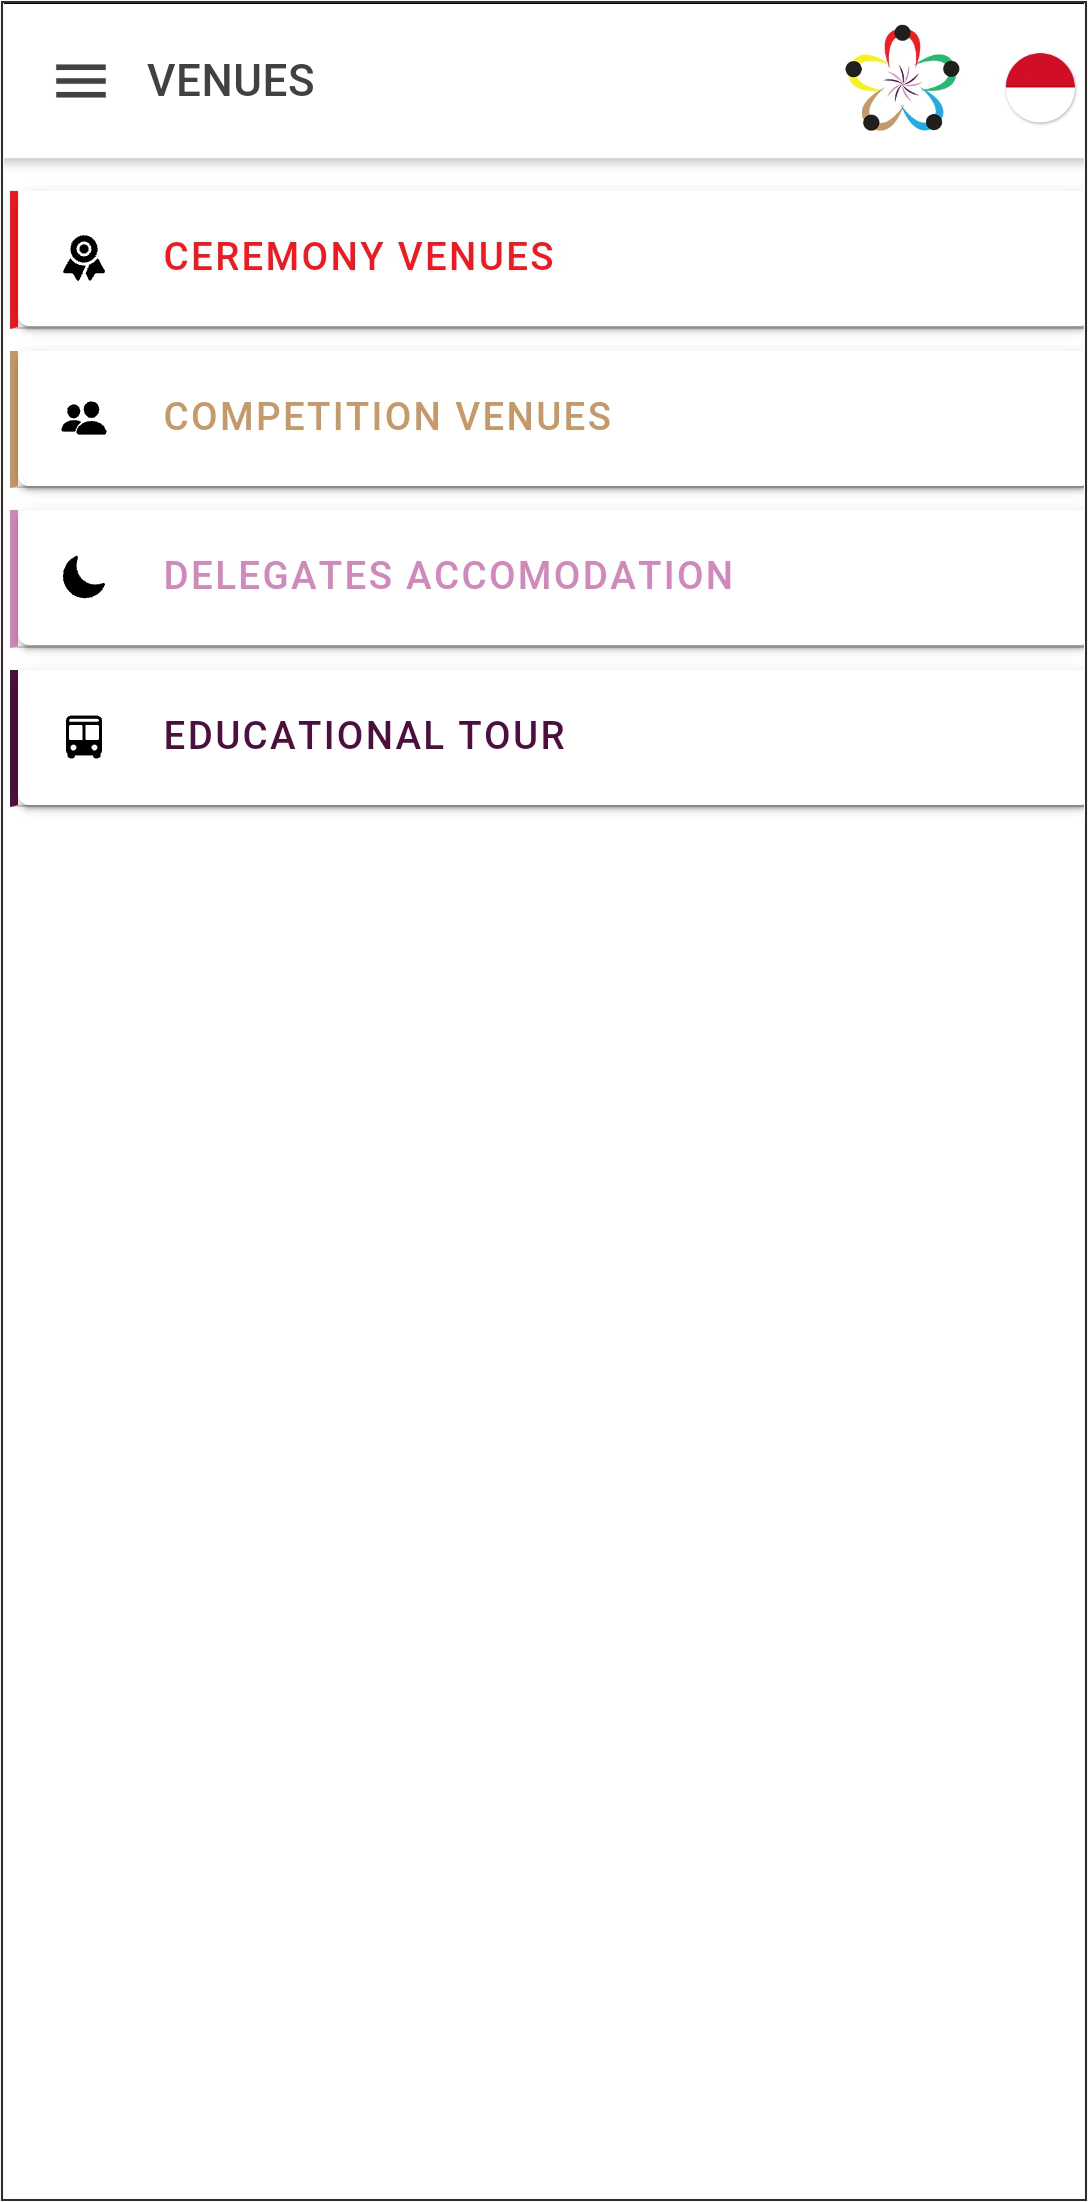
\includegraphics[width=\textwidth]{Gambar/SSVenues.png}
         \caption{\textit{Venues Page} Terbaru}
         \label{fig:ssVenue}
     \end{subfigure}
     \hspace*{0.5in}
     \begin{subfigure}[b]{0.3\textwidth}
         \centering
         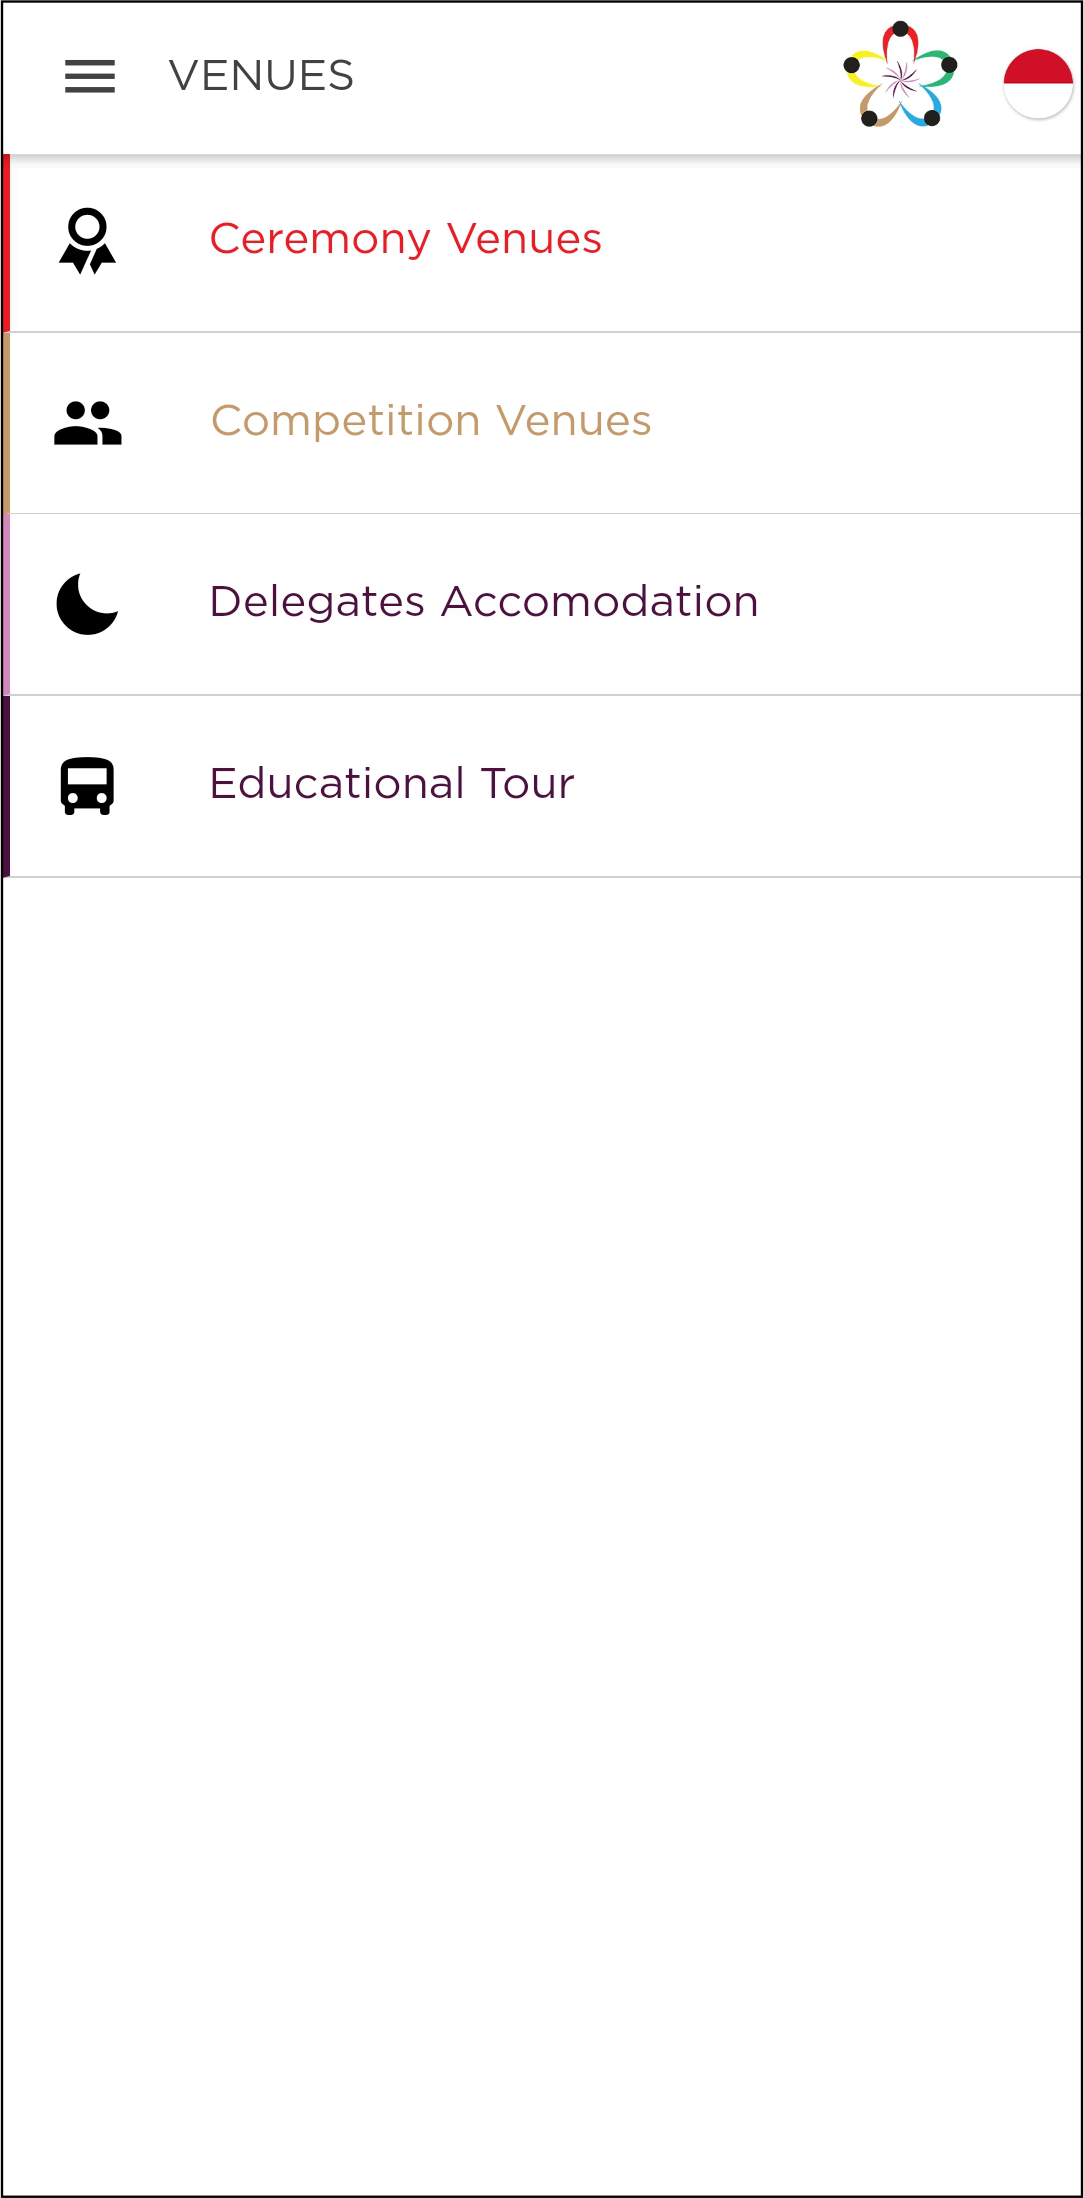
\includegraphics[width=\textwidth]{Gambar/VenuePage.png}
         \caption{\textit{Venues Page} Terdahulu}
         \label{fig:ssVenueOld}
     \end{subfigure}
        \caption{Tangkapan Layar Halaman \textit{Venues} Aplikasi WSDC 2017 Bali}
        \label{fig:ssApk1}
\end{figure}

\begin{figure}[H]
     \centering
     \begin{subfigure}[b]{0.3\textwidth}
         \centering
         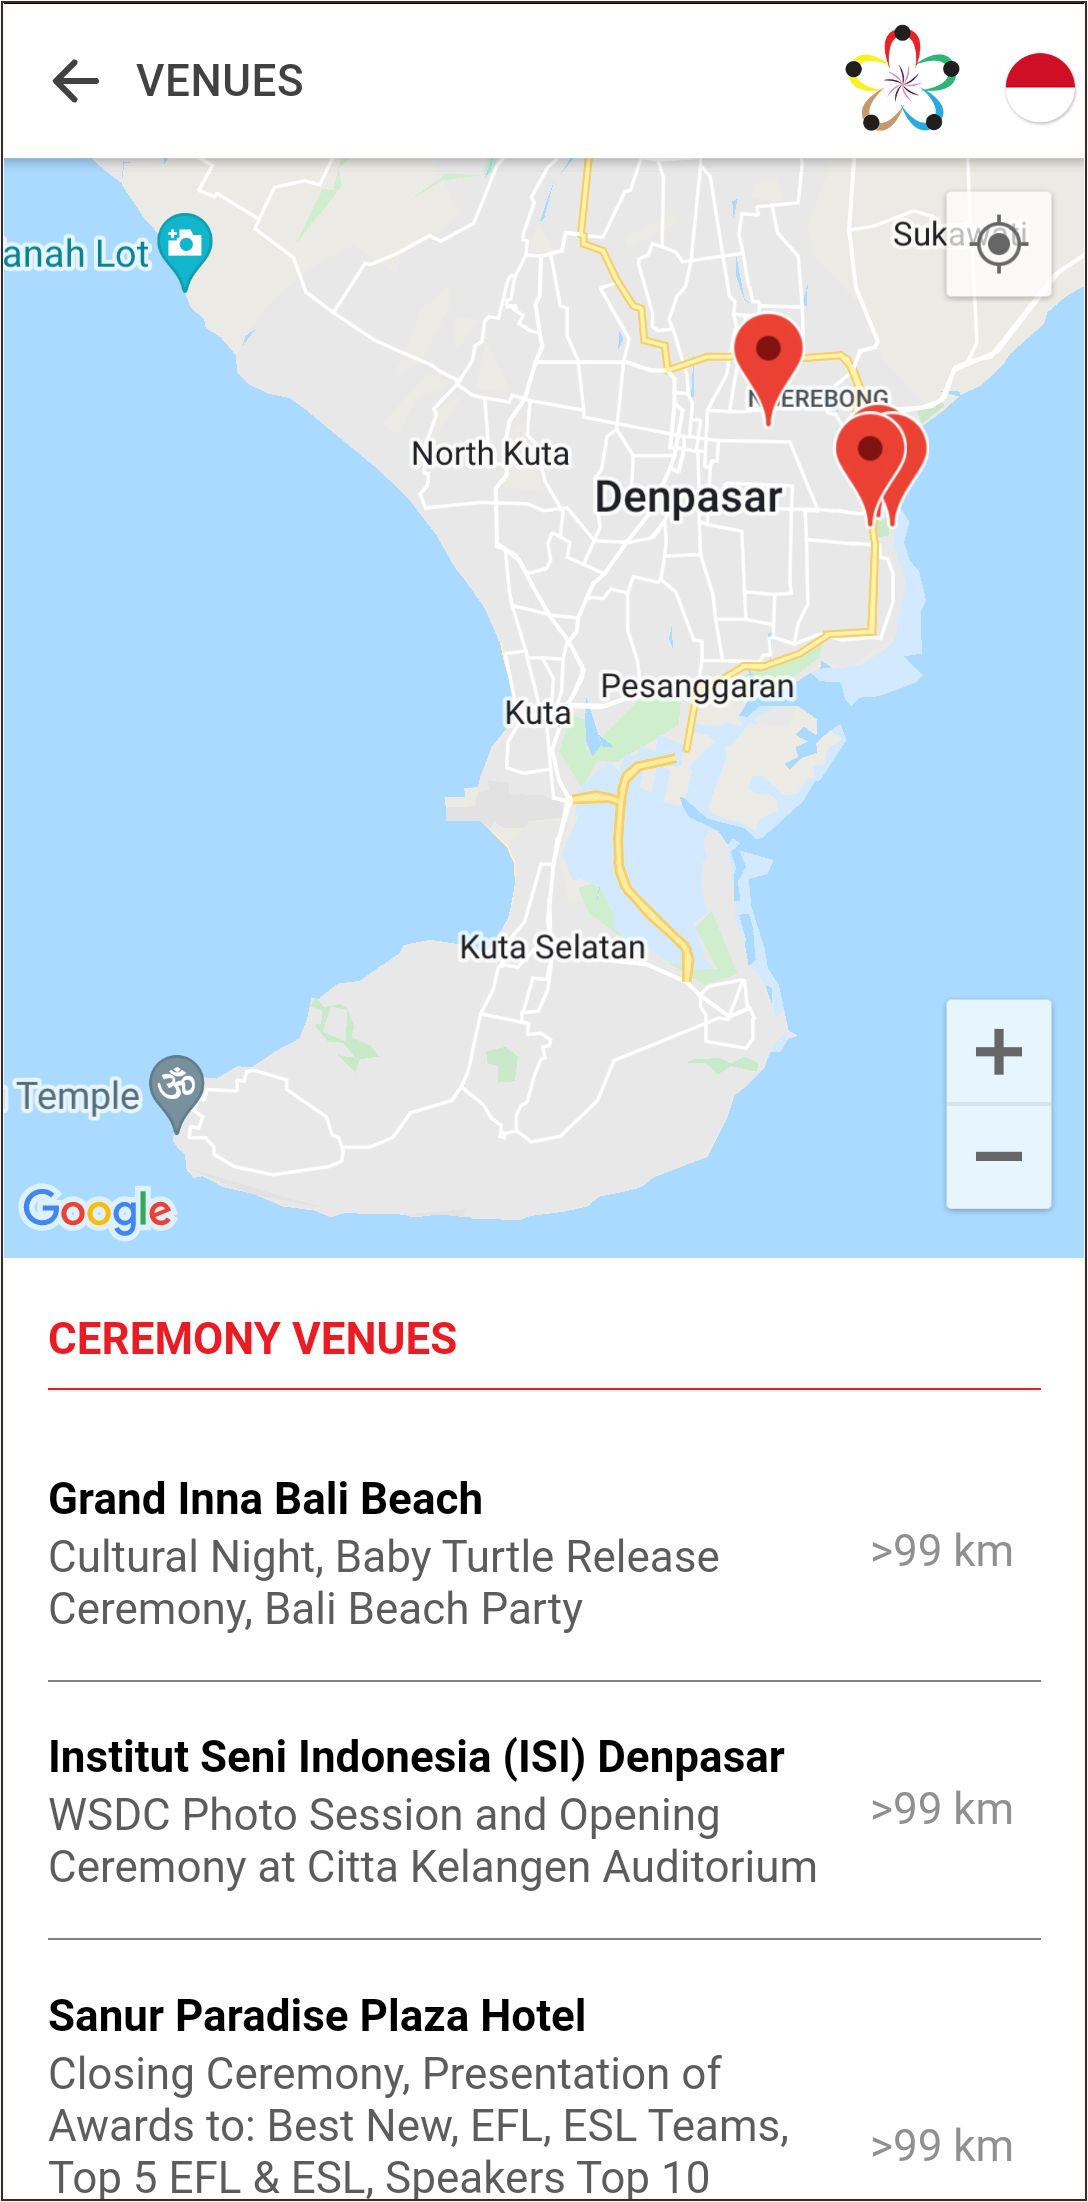
\includegraphics[width=\textwidth]{Gambar/SSVenuesMap.png}
         \caption{\textit{Venues Map Page} Terbaru}
         \label{fig:ssVenueMap}
     \end{subfigure}
     \hspace*{0.5in}
     \begin{subfigure}[b]{0.3\textwidth}
         \centering
         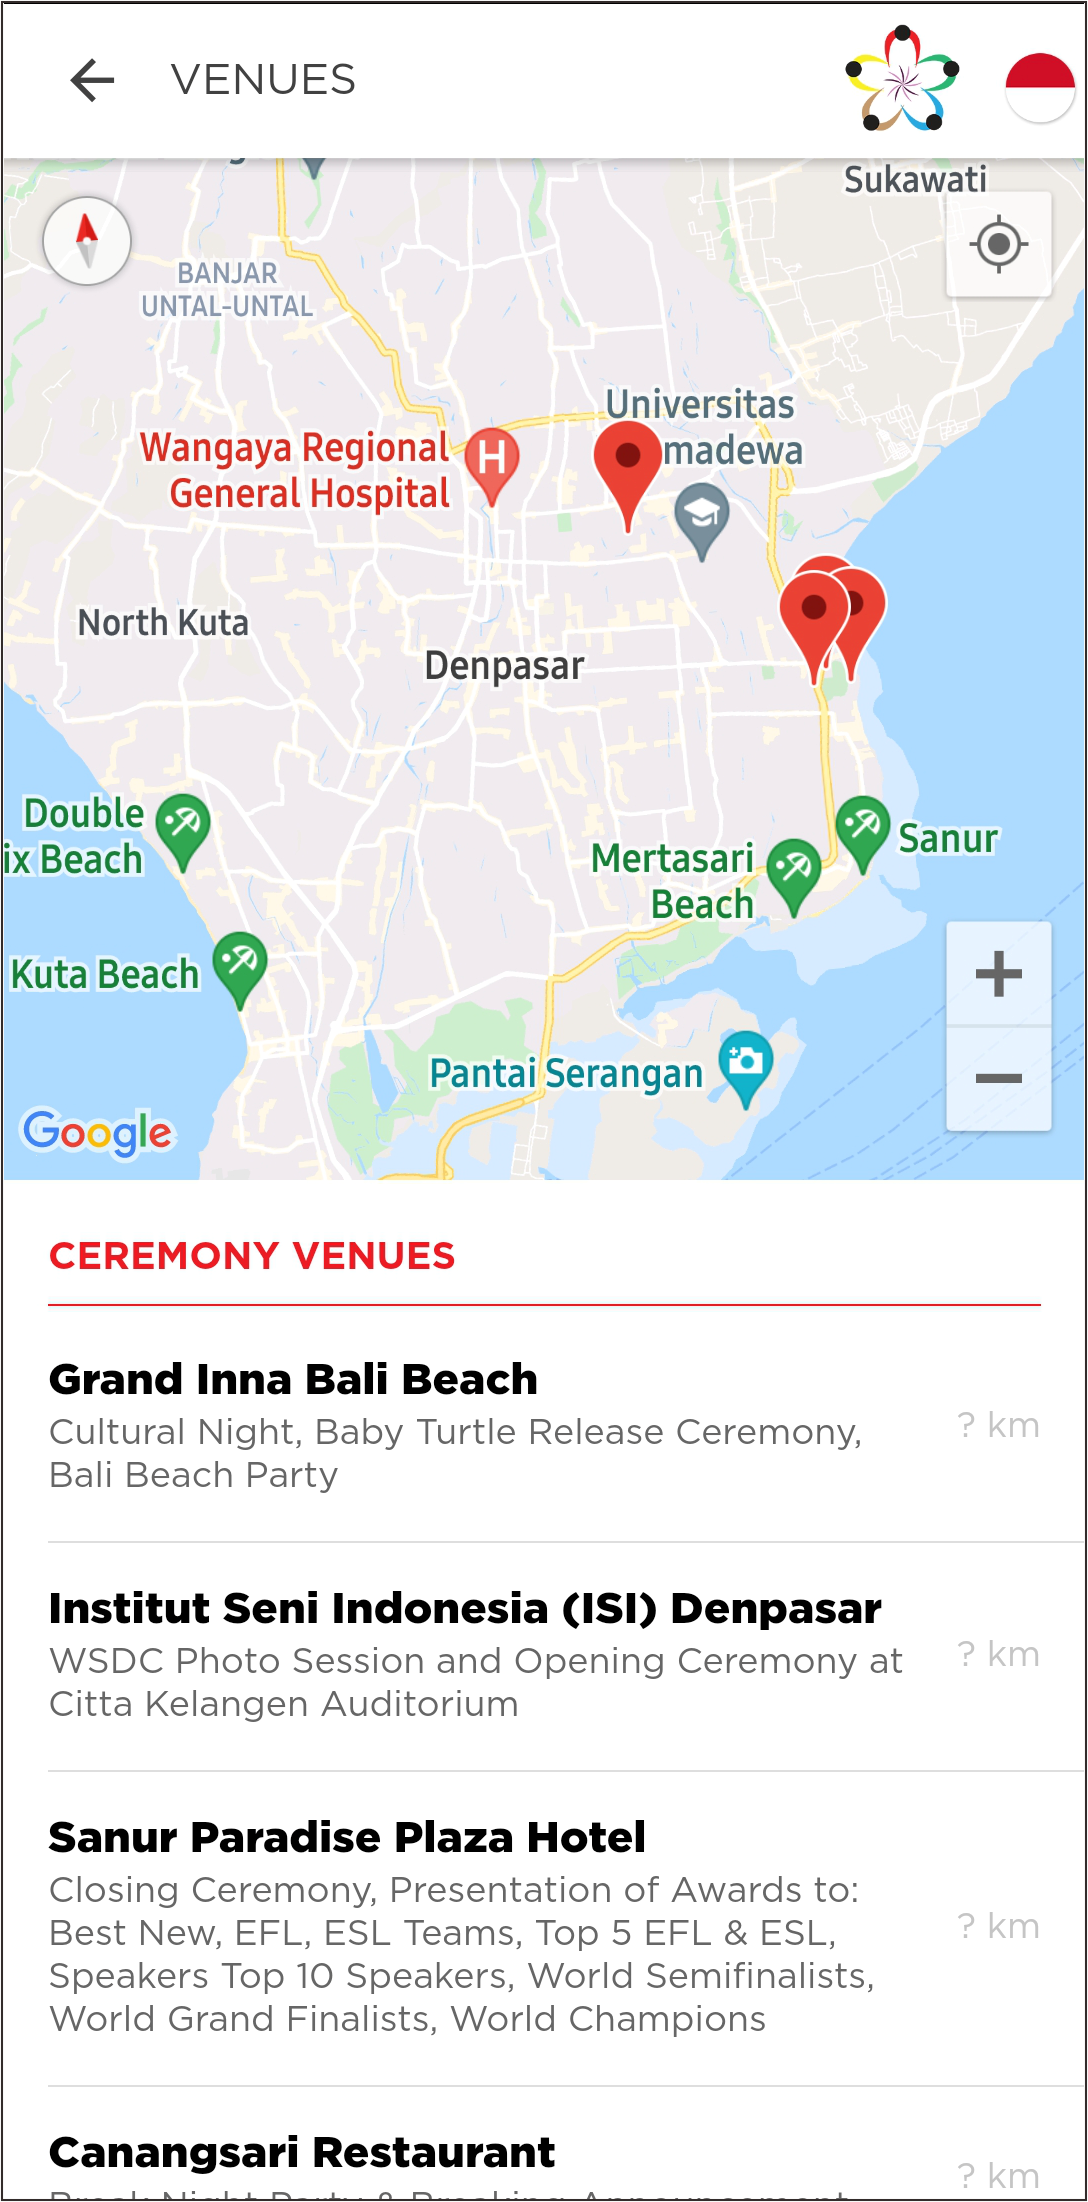
\includegraphics[width=\textwidth]{Gambar/VenuesMapPage.png}
         \caption{\textit{Venues Map Page} Terdahulu}
         \label{fig:ssVenueMapOld}
     \end{subfigure}
        \caption{Tangkapan Layar Halaman \textit{Venues Map} Aplikasi WSDC 2017 Bali}
        \label{fig:ssApk1}
\end{figure}

\section{Pengujian}
\label{sec:pengujian}

\subsection{Pengujian Fungsional}
\label{subsec:pengujianFungsional}

Pengujian fungsional dilakukan untuk mengetahui kesesuaian reaksi perangkat lunak dengan reaksi yang diharapkan berdasarkan aksi pengguna terhadap perangkat lunak. Perangkat yang digunakan untuk melakukan pengujian fungsional ini adalah sebuah perangkat emulator dari Android Studio yaitu Google Pixel 5 dengan versi Android 11, sebuah perangkat emulator Nox Player dengan versi Android 7.1.2, dan sebuah \textit{smartphone} milik penulis yaitu Xiaomi Redmi Note 9 dengan versi Android 11. Tabel~\ref{table:tabelPengujianFungsional} merupakan hasil dari 20 tes kasus yang diujikan.

\begin{table}[H]
\caption{Tabel Pengujian Fungsional}
\label{table:tabelPengujianFungsional}
\begin{tabular}{|p{0.3cm}|p{5.7cm}|p{5.7cm}|p{3cm}|}
\hline
No & Aksi Pengguna                                                                      & Reaksi yang diharapkan                                                               & Reaksi Perangkat Lunak \\ \hline
1  & Pengguna menjalankan aplikasi                                                      & Splash Screen ditampilkan dan aplikasi menampilkan halaman home                      & Sesuai                 \\ \hline
2  & Pengguna menekan tombol hamburger button di pojok kiri atas aplikasi               & Sidemenu terbuka menampillkan menu                                                    & Sesuai                 \\ \hline
3  & Pengguna melakukan swipe dari kiri layar ke kanan layar                            & Sidemenu terbuka menampilkan menu                                                     & Sesuai                 \\ \hline
4  & Pengguna memilih menu Announcements pada Sidemenu                                   & Aplikasi menampilkan halaman Announcements                                         & Sesuai                 \\ \hline
5  & Pengguna memilih menu Home pada Sidemenu                                            & Aplikasi menampilkan halaman Home                                                    & Sesuai                 \\ \hline
6  & Pengguna menekan tombol read more pada Home                                        & Aplikasi mengarahkan pengguna untuk melihat newsletter                               & Sesuai                 \\ \hline
7  & Pengguna menekan card Latest Announcements                                         & Aplikasi mengarahkan pengguna ke halaman Announcements                                & Sesuai                 \\ \hline
8  & Pengguna memilih menu Schedule pada Sidemenu                                        & Aplikasi menampilkan halaman Schedule                                                & Sesuai                 \\ \hline
9  & Pengguna menekan tombol hari dan tanggal pada halaman Schedule                     & Aplikasi menampilkan jadwal yang ada pada hari dan tanggal yang dipilih              & Sesuai                 \\ \hline
10 & Pengguna melakukan swipe secara vertical baik dari kiri ke kanan maupun sebaliknya pada halaman Schedule & Aplikasi menampilkan jadwal yang ada pada hari dan tanggal sebelum maupun sesudahnya & Sesuai                 \\ \hline
11 & Pengguna memilih menu Venues pada Sidemenu                                          & Aplikasi menampilkan halaman Venues                                                  & Sesuai                 \\ \hline
12 & Pengguna memilih kategori venues pada halaman Venues                               & Aplikasi menampilkan halaman Venues Map yang berisi peta dan lokasi venues           & Sesuai                 \\ \hline
13 & Pengguna menekan tombol lokasi pada map                                            & Aplikasi menampilkan lokasi pengguna pada map dengan titik biru                      & Sesuai                 \\ \hline
14 & Pengguna menekan tombol + pada map                                                 & Aplikasi melakukan zoom in pada map                                                  & Sesuai                 \\ \hline
\end{tabular}
\end{table}

\begin{table}[H]
\caption{Lanjutan Tabel Pengujian Fungsional dari Halaman Sebelumnya}
\label{table:tabelPengujianFungsional}
\begin{tabular}{|p{0.3cm}|p{5.7cm}|p{5.7cm}|p{3cm}|}
\hline
No & Aksi Pengguna                                                                      & Reaksi yang diharapkan                                                               & Reaksi Perangkat Lunak \\ \hline
15 & Pengguna menekan tombol – pada map                                                 & Aplikasi melakukan zoom out pada map                                                 & Sesuai                 \\ \hline
16 & Pengguna menekan nama lokasi venues                                                & Aplikasi melakukan zoom in mengarah ke lokasi yang dituju pada map                   & Sesuai                 \\ \hline
17 & Pengguna memilih menu Draw pada Sidemenu                                            & Aplikasi menampilkan halaman Draw                                                    & Sesuai                 \\ \hline
18 & Pengguna memilih menu Result pada Sidemenu                                          & Aplikasi menampilkan halaman Result                                                  & Sesuai                 \\ \hline
19 & Pengguna memilih menu Info pada Sidemenu                                            & Aplikasi menampilkan halaman Info                                                    & Sesuai                 \\ \hline
20 & Pengguna menekan nomor telepon pada halama info                                    & Aplikasi mengarahkan pengguna ke aplikasi pemanggilan                                & Sesuai                 \\ \hline
\end{tabular}
\end{table}
\subsection{Pengujian Eksperimental}
\label{subsec:pengujianEksperimental}

Pengujian eksperimental dilakukan terhadap pengguna \textit{smartphone} dengan sistem operasi Android. Metode pengujian dilakukan dengan cara menyebarkan aplikasi yang dapat diunduh melalui Google Drive~\footnote{Tautan Google Drive aplikasi WSDC 2017 Bali dengan Ionic 6 yang diujikan kepada responden: \url{https://drive.google.com/file/d/1Np29U2dG58Pryp1cbrs-M3XfUcm39cSZ/view?usp=sharing}}. Kemudian, pengguna diminta untuk mengunduh dan menjalankan aplikasi tersebut. Selain itu, pengguna juga diminta untuk mengunduh aplikasi WSDC 2017 Bali terdahulu melalui Google Play Store~\footnote{Tautan Google Play Store aplikasi WSDC 2017 Bali terdahulu: \url{https://play.google.com/store/apps/details?id=org.wsdc2017indonesia.app}} dan menjalankannya. Setelah itu pengguna diminta untuk membandingkan kedua aplikasi tersebut, dan mengisi beberapa pertanyaan terkait pengalaman menggunakan aplikasi WSDC 2017 Bali melalui Google Form. Berikut ini merupakan pertanyaan dan rangkuman jawaban dari hasil pengujian eksperimental terhadap sembilan responden sebagai berikut:

\begin{enumerate}
	\item \textbf{Apa versi Android smartphone Anda?} \\
	Seorang responden menjawab versi Android 5.1, seorang menjawab versi Android 8.0, seorang menjawab versi Android 8.1, seoarang menjawab versi Android 10, dan empat orang menjawab versi Android 11.
	\item \textbf{Saat pertama kali membuka aplikasi, apakah aplikasi WSDC 2017 Bali terbaru menampilkan logo WSDC?} \\
	Semua responden menjawab aplikasi WSDC 2017 Bali terbaru menampilkan logo WSDC.
	\item \textbf{Apakah semua halaman memilki isi nya masing-masing, dan tidak ada halaman yang isinya kosong?} \\
	Semua responden menjawab tidak ada halaman yang tidak memiliki isi.
	\item \textbf{Apakah tombol GPS, \textit{zoom in}, \textit{zoom out}, dan lokasi \textit{venues} yang terdapat pada menu \textit{Venues} dapat berfungsi dengan baik?} \\
	Semua responden menjawab semua tombol berfungsi dengan normal.
	\newpage
	\item \textbf{Apakah Anda mengalami \textit{crash}, \textit{forced close}, atau kendala lain saat menggunakan aplikasi WSDC 2017 Bali terbaru?} \\
	Sebanyak delapan responden menjawab tidak ada crash, forced close, atau kendala lain saat menggunakan aplikasi WSDC 2017 Bali terbaru, dan ada satu responden yang menjawab iya, namun tidak menjelaskan kendala apa yang terjadi.
	\item \textbf{Apakah ada perbedaan positif yang signifikan dibandingkan dengan aplikasi terdahulu?} \\
	Dua orang responden berpendapat bahwa tampilan \textit{sidemenu} tampak lebih segar dan menarik. Lalu sebanyak satu responden berpendapat bahwa tampilan \textit{icon} terlihat lebih beragam dan menarik. Kemudian sebanyak empat responden berpendapat bahwa aplikasi WSDC 2017 Bali terbaru dapat dibuka dengan lebih cepat dibandingkan dengan aplikasi terdahulu. Lalu sebanyak satu responden berpendapat bahwa perubahan aplikasi menjadi lebih baik dari sebelumnya, satu responden menjawab perubahan yang terjadi hanya sedikit, dan satu responden menjawab tidak ada perubahan positif yang dirasakan.
	\item \textbf{Apakah ada perbedaan negatif yang signifikan dibandingkan dengan aplikasi terdahulu?} \\
	Sebanyak empat orang responden menjawab bahwa tidak ada perubahan negatif pada aplikasi WSDC 2017 Bali terbaru. Seorang responden menjawab \textit{font} tulisan lebih kaku, dan halaman \textit{draw} kualitasnya terlihat lebih rendah dibandingkan aplikasi terdahulu. Lalu seorang responden menjawab tampilan pada aplikasi yang terbaru dari menu yang ada di masing-masing \textit{Venues} sedikit aneh, karena nama tempat dan alamatnya saling berdekatan tanpa ada jarak spasi. Dan seorang responden menjawab pemakaian aplikasi terbaru lebih boros.
	\item \textbf{Secara keseluruhan, dengan skala 1-5, seberapa baik aplikasi WSDC 2017 Bali terbaru dibandingkan dengan aplikasi terdahulu?} \\
	Seorang responden menjawab netral dengan skala 3, enam orang responden menjawab dengan skala 4, dan dua orang responden menjawab aplikasi WSDC 2017 Bali lebih baik dibandingkan aplikasi terdahulu dengan skala 5.
	\item \textbf{Apakah Anda lebih memilih menggunakan aplikasi WSDC 2017 Bali terdahulu, atau yang terbaru?} \\
	Sebanyak delapan responden memilih untuk menggunakan aplikasi WSDC 2017 Bali terbaru, sedangkan satu responden memilih untuk menggunakan aplikasi WSDC 2017 Bali terdahulu.
	\item \textbf{Apakah terdapat kritik dan saran terhadap aplikasi WSDC 2017 Bali terbaru?} \\
	Terdapat beberapa kritik dan saran dari responden sebagai berikut:
	\begin{enumerate}
		\item Dapat memilih font yang lebih menarik dan nyaman untuk dibaca.
		\item Pada halaman \textit{Result} diharapkan agar memiliki yang tampilan lebih menarik lagi.
		\item Ukuran aplikasi bisa dikecilkan.
		\item Pada halaman \textit{venues} dimana tulisan headline dari list map dijauhkan sedikit dari tulisan body karena terlalu dekat.
	\end{enumerate}

\end{enumerate}
